% Soubory musí být v kódování, které je nastaveno v příkazu \usepackage[...]{inputenc}

\documentclass[%
%  draft,    				  % Testovací překlad
  12pt,       				% Velikost základního písma je 12 bodů
  a4paper,    				% Formát papíru je A4
%  oneside,      			% Jednostranný tisk (výchozí)
%% Z následujicich voleb lze použít maximálně jednu:
%	dvipdfm  						% výstup bude zpracován programem 'dvipdfm' do PDF
%	dvips	  						% výstup bude zpracován programem 'dvips' do PS
%	pdftex							% překlad bude proveden programem 'pdftex' do PDF (výchozí)
	unicode,						% Záložky a informace budou v kódování unicode
%% Z následujících voleb lze použít jen jednu:
%english,            % originální jazyk je angličtina
czech              % originální jazyk je čeština (výchozí)
%slovak,             % originální jazyk je slovenčina
]{report}				    	% Dokument třídy 'zpráva'

\usepackage[utf8]		%	Kódování zdrojových souborů je v UTF-8
	{inputenc}					% Balíček pro nastavení kódování zdrojových souborů

\usepackage{graphicx} % Balíček 'graphicx' pro vkládání obrázků
											% Nutné pro vložení log školy a fakulty

\usepackage[
	nohyperlinks				% Nebudou tvořeny hypertextové odkazy do seznamu zkratek
]{acronym}						% Balíček 'acronym' pro sazby zkratek a symbolů
											% Nutné pro použití prostředí 'seznamzkratek' balíčku 'thesis'

\usepackage[
	breaklinks=true,		% Hypertextové odkazy mohou obsahovat zalomení řádku
	hypertexnames=false % Názvy hypertextových odkazů budou tvořeny
											% nezávisle na názvech TeXu
]{hyperref}						% Balíček 'hyperref' pro sazbu hypertextových odkazů
											% Nutné pro použití příkazu 'nastavenipdf' balíčku 'thesis'

\usepackage{pdfpages} % Balíček umožňující vkládat stránky z PDF souborů
                      % Nutné při vkládání titulních listů a zadání přímo
                      % ve formátu PDF z informačního systému

\usepackage{enumitem} % Balíček pro nastavení mezerování v odrážkách
  \setlist{topsep=0pt,partopsep=0pt,noitemsep}

\usepackage{cmap} 		% Balíček cmap zajišťuje, že PDF vytvořené `pdflatexem' je
											% plně "prohledávatelné" a "kopírovatelné"

\usepackage{upgreek}	% Balíček pro sazbu stojatých řeckých písmem
											% např. stojaté pí: \uppi
											% např. stojaté mí: \upmu (použitelné třeba v mikrometrech)
											% pozor, grafická nekompatibilita s fonty typu Computer Modern!

\usepackage{dirtree}		% sazba adresářové struktury

\usepackage[formats]{listings}	% Balíček pro sazbu zdrojových textů
\lstset{
%	Definice jazyka použitého ve výpisech
%    language=[LaTeX]{TeX},	% LaTeX
%	language={Matlab},		% Matlab
	language={C},           % jazyk C
    basicstyle=\ttfamily,	% definice základního stylu písma
    tabsize=2,			% definice velikosti tabulátoru
    inputencoding=utf8,         % pro soubory uložené v kódování UTF-8
    %inputencoding=cp1250,      % pro soubory uložené ve standardním kódování Windows CP1250
		columns=fixed,  %flexible,
		fontadjust=true %licovani sloupcu
    extendedchars=true,
    literate=%  definice symbolů s diakritikou
    {á}{{\'a}}1
    {č}{{\v{c}}}1
    {ď}{{\v{d}}}1
    {é}{{\'e}}1
    {ě}{{\v{e}}}1
    {í}{{\'i}}1
    {ň}{{\v{n}}}1
    {ó}{{\'o}}1
    {ř}{{\v{r}}}1
    {š}{{\v{s}}}1
    {ť}{{\v{t}}}1
    {ú}{{\'u}}1
    {ů}{{\r{u}}}1
    {ý}{{\'y}}1
    {ž}{{\v{z}}}1
    {Á}{{\'A}}1
    {Č}{{\v{C}}}1
    {Ď}{{\v{D}}}1
    {É}{{\'E}}1
    {Ě}{{\v{E}}}1
    {Í}{{\'I}}1
    {Ň}{{\v{N}}}1
    {Ó}{{\'O}}1
    {Ř}{{\v{R}}}1
    {Š}{{\v{S}}}1
    {Ť}{{\v{T}}}1
    {Ú}{{\'U}}1
    {Ů}{{\r{U}}}1
    {Ý}{{\'Y}}1
    {Ž}{{\v{Z}}}1
}

%% Nastavení českého jazyka při sazbě v češtině.
% Pro sazbu češtiny je možné použít mezinárodní balíček 'babel', jenž
% použití doporučujeme pro nové instalace (MikTeX2.8,TeXLive2009), nebo
% národní balíček 'czech', který doporučujeme ve starších instalacích.
% Balíček 'babel' bude správně fungovat pouze ve spojení s programy
% 'latex', 'pdflatex', zatímco balíček 'czech' bude fungovat ve spojení
% s programy 'cslatex', 'pdfcslatex'.
% Varianta A:
\usepackage    				
  {babel}             % Balíček pro sazbu různojazyčných dokumentů; kompilovat (pdf)latexem!
  										% převezme si z parametrů třídy správný jazyk
\usepackage{lmodern}	% vektorové fonty Latin Modern, nástupce půvoních Knuthových Computern Modern fontů
\usepackage{textcomp} % Dodatečné symboly
\usepackage[T1]{fontenc}  % Kódování fontu - mj. kvůli správným vzorům pro dělení slov
% Varianta B:
%\usepackage{czech}   % Alternativní balíček pro sazbu v českém jazyce, kompilovat (pdf)cslatexem!

\usepackage[%
%% Z následujících voleb lze použít pouze jednu
% left,               % Rovnice a popisky plovoucich objektů budou %zarovnány vlevo
  center,             % Rovnice a popisky plovoucich objektů budou zarovnány na střed (vychozi)
%% Z následujících voleb lze použít pouze jednu
diploma						%	sazba zprávy semestrálního projektu
%bachelor						%	sazba bakalářské práce
%diploma						 % sazba diplomové práce
%treatise            % sazba pojednání o dizertační práci
%phd                 % sazba dizertační práce
]{thesis}             % Balíček pro sazbu studentských prací
                      % Musí být vložen až jako poslední, aby
                      % ostatní balíčky nepřepisovaly jeho příkazy

\usepackage{amsmath}
\usepackage{mathtools}
\usepackage{alize} %moje styly

%\usepackage{listings}
%\lstset {breaklines=true}
\usepackage{fancyvrb}

\usepackage{rotating}
\usepackage{multirow}

%%%%%%%%%%%%%%%%%%%%%%%%%%%%%%%%%%%%%%%%%%%%%%%%%%%%%%%%%%%%%%%%%
%%%%%%      Definice informací o dokumentu             %%%%%%%%%%
%%%%%%%%%%%%%%%%%%%%%%%%%%%%%%%%%%%%%%%%%%%%%%%%%%%%%%%%%%%%%%%%%

%% Název práce:
%  První parametr je název v originálním jazyce,
%  druhý je překlad v angličtině nebo češtině (pokud je originální jazyk angličtina)
\nazev{Paralelizace Goertzelova algoritmu}{Parallelization of Goertzel algorithm}

%% Jméno a příjmení autora ve tvaru
%  [tituly před jménem]{Křestní}{Příjmení}[tituly za jménem]
\autor[Bc.]{Zdeněk}{Skulínek}

%% Jméno a příjmení vedoucího včetně titulů
%  [tituly před jménem]{Křestní}{Příjmení}[tituly za jménem]
% Pokud vedoucí nemá titul za jménem, smažte celý řetězec '[...]'
\vedouci[Ing.]{Petr}{Sysel}[Ph.D.]

%% Jméno a příjmení oponenta včetně titulů
%  [tituly před jménem]{Křestní}{Příjmení}[tituly za jménem]
% Pokud nemá titul za jménem, smažte celý řetězec '[...]'
% Uplatní se pouze v prezentaci k obhajobě
\oponent[prof.\ Ing.]{Zdeněk}{Smékal}[CSc.]

%% Označení oboru studia
% První parametr je obor v originálním jazyce,
% druhý parametr je překlad v angličtině nebo češtině
\oborstudia{Teleinformatika}{Teleinformatics}

%% Označení ústavu
% První parametr je název ústavu v originálním jazyce,
% druhý parametr je překlad v angličtině nebo češtině
\ustav{Ústav telekomunikací}{Department of Telecommunications} 

%% Rok obhajoby
\rok{Rok}
\datum{7.\,6.\,2017} % Uplatní se pouze v prezentaci k obhajobě

%% Místo obhajoby
% Na titulních stránkách bude automaticky vysázeno VELKÝMI písmeny
\misto{Brno}

%% Abstrakt
\abstrakt{
Technické problémy znemožňují neustále zvyšovat hodinové frekvence procesorů.
Jejich výkon tak v současné době roste díky zvyšování počtu jader.
To s sebou přináší nutnost nových přístupů pro programování takovýchto paralelních systémů.
Tato práce ukazuje, jak využít paralelismus k číslicovému zpracování signálu. Jako příklad zde bude uvedena implementace Geortzelova algoritmu s využitím výpočetního výkonu grafického čipu.
}{
Technical problems make impossible steadily increase processor's clock frequency.
Their power are currently growing due to increasing number of cores.
It brings need for new approaches in programming such parallel systems.
This thesis shows how to use paralelism in digital signal processing.
As an example, it will be presented here
implementation of the Geortzel's algorithm using the processing power of the graphics chip.
}

%% Klíčová slova
\klicovaslova{Goertzelův algoritmus, zpracování signálu, openCL, paralelní výpočet, GPU}%
	{Goertzel's algorithm, signal processing, openCL, parallel computing, GPU}

%% Poděkování
\podekovanitext{Rád bych poděkoval vedoucímu diplomové práce panu Ing.~Petru Syslovi, Ph.D.\ za odborné vedení, konzultace, trpělivost a podnětné návrhy k~práci.}  % do tohoto souboru doplňte údaje o sobě, o názvu práce...

%%%%%%%%%%%%%%%%%%%%%%%%%%%%%%%%%%%%%%%%%%%%%%%%%%%%%%%%%%%%%%%%%%%%%%%%

%%%%%%%%%%%%%%%%%%%%%%%%%%%%%%%%%%%%%%%%%%%%%%%%%%%%%%%%%%%%%%%%%%%%%%%%
%%%%%%     Nastavení polí ve Vlastnostech dokumentu PDF      %%%%%%%%%%%
%%%%%%%%%%%%%%%%%%%%%%%%%%%%%%%%%%%%%%%%%%%%%%%%%%%%%%%%%%%%%%%%%%%%%%%%
%% Při vloženém balíčku 'hyperref' lze použít příkaz '\nastavenipdf'
\nastavenipdf
%  Nastavení polí je možné provést také ručně příkazem:
%\hypersetup{
%  pdftitle={Název studentské práce},    	% Pole 'Document Title'
%  pdfauthor={Autor studenstké práce},   	% Pole 'Author'
%  pdfsubject={Typ práce}, 						  	% Pole 'Subject'
%  pdfkeywords={Klíčová slova}           	% Pole 'Keywords'
%}
%%%%%%%%%%%%%%%%%%%%%%%%%%%%%%%%%%%%%%%%%%%%%%%%%%%%%%%%%%%%%%%%%%%%%%%

%%%%%%%%%%%%%%%%%%%%%%%%%%%%%%%%%%%%%%%%%%%%%%%%%%%%%%%%%%%%%%%%%%%%%%%
%%%%%%%%%%%       Začátek dokumentu               %%%%%%%%%%%%%%%%%%%%%
%%%%%%%%%%%%%%%%%%%%%%%%%%%%%%%%%%%%%%%%%%%%%%%%%%%%%%%%%%%%%%%%%%%%%%%
\begin{document}


%% Vložení desek generovaných informačním systémem
\includepdf[pages=1,offset=19mm 0mm]%
  {pdf/student-desky}% název souboru nesmí obsahovat mezery!
% nebo vytvoření desek z balíčku
%\vytvorobalku
\setcounter{page}{1} %resetovani citace stranek - desky se necisluji

%% Vložení titulního listu generovaného informačním systémem
\includepdf[pages=1,offset=19mm 0mm]%
  {pdf/student-titulka}% název souboru nesmí obsahovat mezery!
% nebo vytvoření titulní stránky z balíčku
%\vytvortitulku
   
%% Vložení zadání generovaného informačním systémem
\includepdf[pages=1,offset=19mm 0mm]%
  {pdf/student-zadani}% název souboru nesmí obsahovat mezery!
% nebo lze vytvořit prázdný list příkazem ze šablony
%\stranka{}%
%	{\sffamily\Huge\centering ZDE VLOŽIT LIST ZADÁNÍ}%
%	{\sffamily\centering Z~důvodu správného číslování stránek}

%% Vysázení stránky s abstraktem
\vytvorabstrakt

%% Vysázení prohlaseni o samostatnosti
\vytvorprohlaseni

%% Vysázení poděkování
\vytvorpodekovani

%% Vysázení poděkování projektu SIX
% ----------- zakomentujte pokud neodpovida realite
%\vytvorpodekovaniSIX

%% Vysázení obsahu
\obsah

%% Vysázení seznamu obrázků
\seznamobrazku

%% Vysázení seznamu tabulek
\seznamtabulek

%% Vysázení seznamu výpisů
%\lstlistoflistings



%
%\input{Zaver}% nutné





%% Vložení souboru 'text/uvod.tex' s úvodem
\chapter*{Úvod}
\phantomsection
\addcontentsline{toc}{chapter}{Úvod}


Moderní architektury procesorů využívají paralelismus jako důležitou cestu
ke zvýšení výpočetního výkonu. Řeší se tím zejména technické problémy při
zvyšování hodinových kmitočtů, kde se naráží na fyzikální limity.
\zk{zkCPU} zvyšují výkon přidáváním jader. \zk{zkGPU} 
se vyvinula z pevně dané renderovací funkcionality
do podoby paralelních programovatelných procesorů.	Protože dnešní počítače
často obsahují vícejádrové \zk{zkCPU} a \zk{zkGPU} a další procesory,
je velmi důležité vzít v úvahu specifika programování pro takovéto
 paralelní systémy.

Vytváření aplikací pro vícejádrové procesory je oproti tradičním jednojádrovým
aplikacím složitější, neboť je potřeba použít zcela jiného přístupu. Více procesorové systémy jsou navíc silně platformně a hardwarově závislé, což činí jejich programování obtížnější.

Mým úkolem je ukázat možnosti dnešních počítačů při zpracování signálu.
Jako modelový příklad mám implementovat \emph{Goertzelův algoritmus}, což je
číslicový filtr, na jehož vstupu je číslicový signál a parametr $k$, udávající  konkrétní harmonickou  složku spektra signálu navzorkovaného s kmitočtem $f_{vz}$. Jeho výstupem je pak jediná hodnota vyjadřující amplitudu na určitém kmitočtu.

Paralelizovaný Goertzelův algoritmus představím na své aplikaci nazvané \emph{Sound Analyzer}, která počítá libovolná počet složek spektra v reálném čase a zobrazuje výsledné spektrum g grafickém prostředí.

Tato práce zažíná představením \emph{Goertzelova algoritmu} \ref{kap:goertzeluvalgoritmus}. Na jejím základě jsem napsal kapitolu \emph{možnosti řešení}\ref{kap:moznostireseni}, ve které uvádím techniky řešení a odvozuji vzorce, které použiji pro sestavení programu \emph{Sound Analyzer}. Kapitola následující je pak malým úvodem do problematiky paralelizace. Řešení diplomové práce, program \emph{Sound Analyzer} \ref{kap:programsoundanalyzer} včetně jeho součástí, koncepce a licence jsou uvedeny v kapitole \ref{kap:programsoundanalyzer}. Z~popisu programu přecházím do popisu použitých knihoven\ref{kap:libraries} a vysvětlení, proč jsem využil zrovna tyto.
V poslední kapitole \emph{měření přínosu} \ref{kap:measurement} odpovídám na otázku, jaký je přínos využití GPU při zpracování signálu.


\chapter{Goertzelův algoritmus}
\label{kap:goertzeluvalgoritmus}

\section{Diskrétní Fourierova řada}

Máme řadu $N$ hodnot libovolné posloupnosti. Fourier ukázal, že je možno převést
ji na $N$ hodnot nějaké frekvenční charakteristiky. \emph{Diskrétní Fourierova řada} přiřazuje časové periodické posloupnosti periody $N$,
posloupnost spektra, rovněž periodickou a rovněž periody $N$. Následující vzorec pochází z knihy \emph{Systémy a signály} od prof. Smékala\cite{smekal}.

\begin{myequation}
S_p[k] = \sum_{n=0}^{N-1} s_p[n] \eul^{-\jmag  k\frac{2\pi}{N}n},
\end{myequation}
\noindent kde \emph{k} $k.$ hodnota amplitudy ve spektru, nabývá hodnot $0..N-1, N$ je délka sekvence časové posloupnosti i délka spektra \emph{DFŘ}.
Řada má tedy určitý, omezený počet členů.

\section{Diskrétní Fourierova transformace - DFT}


Na rozdíl od \emph{DFŘ}, není obraz \emph{DFT} periodický. \emph{DFT} přiřazuje
časové posloupnosti délky $N$, posloupnost spektra, také délky $N$. S pomocí
\emph{DFŘ} by se vytvořil asi takto:
\begin{itemize}
\item Zperiodizování průběhu $s$, kde $s[n+lN] = s_p[n]$
\item Výpočet DFŘ.
\item Oříznutí spektra na jednorázovou posloupnost. 
\end{itemize}

\emph{DFT} zapisujeme jako

\begin{myequation}
\label{vztah:DFT}
S[k] = \sum_{n=0}^{N-1} s[n] \eul^{-\jmag  k\frac{2\pi}{N}n}.
\end{myequation}

I tento vzorec pochází z knihy prof. Smékala (\cite{smekal}).

\section{Goertzelův algoritmus}

Často je třeba řešit požadavek na zjištění složky spektra u určitém úzkém pásmu kmitočtů. Šlo by samozřejmě spočítat Fourierovou transformací celé spektrum a~vybrat jen ten kmitočet, který je pro nás zajímavý.
Další možností je spočítání jedné hodnoty z definice Fourierovy transformace, tak jako ve vzorci pro DFT (\ref{vztah:DFT}).
Myšlenkou \emph{Goertzelova algoritmu} je k tomuto účelu použít číslicové filtrace.
Goertzel použil druhou kanonickou strukturu (\ref{vztah:2kanonickastruktura}), realizovanou filtrem IIR (na obrázku \ref{obr:2kanonicka}).

\begin{myequation}
\begin{multlined}
\label{vztah:2kanonickastruktura}
v_1[n+1] = v_2[n] \\
v_2[n+1] = \frac{1}{b_2}(x[n]-b_1v_2[n]-b_0v_1[n]) \\
y[n] = a_2v_2[n+1] + a_1v_2[n] +a_0v_1[n] 
\end{multlined}
\end{myequation}

\begin{figure}
  \begin{center}
    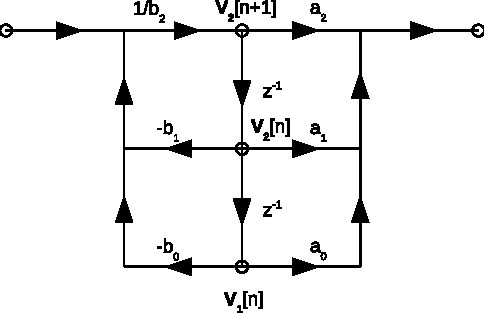
\includegraphics[scale=1]{obr/2kanonickastruktura}
  \end{center}
  \caption{Graf signálových toků druhé kanonické struktury.}
  \label{obr:2kanonicka}
\end{figure}


\section{Odvození Goertzelova algoritmu}

Následující odvození pochází rovněž z knihy prof. Smékala Systémy a signály \cite{smekal}.
\\
 Označme:

\begin{myequation}
\label{vztah:wn}
W_N = \eul^{-\jmag  \frac{2\pi}{N}},
\end{myequation}

pak

\begin{myequation}
\label{vztah:wnrovnost}
(W_N)^{-kN} = (\eul^{-\jmag  \frac{2\pi}{N}})^{-kN} = 1,
\end{myequation}

Protože člen (\ref{vztah:wnrovnost}) je jedna, můžeme s ním vynásobit definiční vztah Fourierovy transformace (\ref{vztah:DFT}), aniž by došlo ke změně.

\begin{myequation}
\begin{multlined}
\label{vztah:geotrzelsk}
S[k] = \sum_{m=0}^{N-1} s[m] W_N^{-kN} = (W_N)^{-kN} \sum_{m=0}^{N-1} s[m] W_N^{-kN} =\\
=\sum_{m=0}^{N-1} s[m] W_N^{-k(N-m)} = \sum_{m=0}^{N-1} s[m] \eul^{-\jmag\frac{2\pi}{N}k(N-m)}
\end{multlined}
\end{myequation}

Konečný tvar vztahu (\ref{vztah:geotrzelsk}) zjevně vypadá jako konvoluce
vstupní posloupnosti $x[n] = s[n]$ s impulsní charakteristikou číslicového filtru typu IIR


\begin{myequation}
\label{vztah:gertzelimpchar}
h[n] =  \eul^{-\jmag  k\frac{2\pi}{N}} = W_N^{-kN} = 1, n = 0,1,2..\infty
\end{myequation}

Impulsní charakteristika má komplexní koeficienty, což je zřejmé i z toho, že
spektrum DFT je také komplexní. Výstupní odezva potom je

\begin{myequation}
\begin{multlined}
\label{vztah:geotrzelyn}
y[n] = x[n]*h[n] = \sum_{m=0}^{\infty} s[m] h[n-m] = \sum_{m=0}^{\infty} s[m] W_N^{-k(n-m)} = \\
\sum_{m=0}^{\infty} s[m] \eul^{-\jmag k\frac{2\pi}{N}(n-m)}
\end{multlined}
\end{myequation}

Tento vzorec (\ref{vztah:geotrzelyn}) je ovšem nekonečná řada. Naštěstí není nutné
počítat do nekonečna, jelikož v hledané spektrální složce je jediný vzorek v čase $N$ roven

\begin{myequation}
\begin{multlined}
\label{vztah:geotrzelopak}
y[N] = \sum_{m=0}^{\infty} s[n] \eul^{-\jmag k\frac{2\pi}{N}(N-m)} =
\sum_{m=0}^{\infty} s[n] \eul^{-\jmag k\frac{2\pi}{N}N} \eul^{-\jmag k\frac{2\pi}{N}m} =
\sum_{m=0}^{N-1} s[n] \eul^{-\jmag k\frac{2\pi}{N}m} =\\
 S[k]
\end{multlined}
\end{myequation}

Přenosová charakteristika filtru typu IIR s impulsní charakteristikou (\ref{vztah:gertzelimpchar}) je prvního řádu

\begin{myequation}
\begin{multlined}
\label{vztah:geotrzelhz}
H(z) = \sum_{n=0}^{\infty} h[n]z^{-n} =  \sum_{n=0}^{\infty} \eul^{-\jmag k\frac{2\pi}{N}n} z^{-n}= \sum_{n=0}^{\infty} ( \eul^{-\jmag k\frac{2\pi}{N}} z^{-1} )^{n} =\\
 \frac{1}{1-\eul^{-\jmag k\frac{2\pi}{N}}z^{-1}} = \frac{z}{z-W_N^{-k}}
\end{multlined}
\end{myequation}

Nevýhodou zcela jistě je skutečnost, že se v přenosové funkci vyskytují komplexní
koeficienty. Následující úprava vztahu (\ref{vztah:geotrzelhz}) tohle řeší. Daň za
možnost práce s jen reálnými čísly je přenosová funkce druhého řádu.

\begin{myequation}
\begin{multlined}
\label{vztah:geotrzelodvoz}
H(z) = \frac{1}{1-W_N^{-k}z^{-1}} = \frac{1}{1-W_N^{-k}z^{-1}} . \frac{1-W_N^{k}z^{-1}}{1-W_N^{k}z^{-1}} =\\
 \frac{1}{1-\eul^{-\jmag k\frac{2\pi}{N}z^{-1}}}
. \frac{1-\eul^{-\jmag  k\frac{2\pi}{N}z^{-1}}}{1-\eul^{-\jmag  k\frac{2\pi}{N}z^{-1}}} =
\frac{1-\eul^{-\jmag  k\frac{2\pi}{N}z^{-1}}}{1 - (\eul^{-\jmag  k\frac{2\pi}{N}+\eul^{-\jmag k\frac{2\pi}{N}})z^{-1} +z^{-2}}} = \\
\frac{1-\eul^{-\jmag  k\frac{2\pi}{N}z^{-1}}}{1-2\cos{k\frac{2\pi}{N}}z^{-1}+z^{-2}} =
\frac{z^{2}-\eul^{-\jmag  k\frac{2\pi}{N}z}}{z^{2}-2\cos{k\frac{2\pi}{N}}z+1} = 
\frac{a_2z^{2}+a_1z+a_0}{b_2z^{2}+b_1z+b_0}
\end{multlined}
\end{myequation}

Výsledek porovnáme se stavovými rovnicemi (\ref{vztah:2kanonickastruktura}) A zjistíme tak následující koeficienty.

\begin{myequation}
\begin{aligned}
\label{vztah:geotrzelkoef}
b_2 &= 1,&&\\
b_1 &= -2\cos{k\frac{2\pi}{N}},&&\\
b_0 &= 1,&&\\
a_2 &= 1,&&\\
a_1 &= -\eul^{-\jmag  k\frac{2\pi}{N}},&&\\
a_0 &= 0
\end{aligned}
\end{myequation}


Jejich dosazením  do (\ref{vztah:2kanonickastruktura}) dostaneme...

\begin{myequation}
\begin{aligned}
\label{vztah:geortzelstavrovnice}
v_1[n+1] &= v_2[n], &&\\
v_2[n+1] &= x[n]+2\cos{k\frac{2\pi}{N}}v_2[n]-v_1[n], &&\\
y[n] &= v_2[n+1] -(\cos{k\frac{2\pi}{N}} -\jmag  \sin{k\frac{2\pi}{N}}) v_2[n], &&\\
\end{aligned}
\end{myequation}


\begin{figure}
  \begin{center}
    
\includegraphics[scale=1]{obr/goertzel}
  \end{center}
  \caption{Graf signálových toků Goertzelova algoritmu ve 2. kanonické struktuře.}
  \label{obr:goertzelova2kanonicka}
\end{figure}

Výhodou této struktury je, že nám stačí ve smyčce počítat jen proměnné
$v_1$ a $v_2$. Výstup $y$ se počítá jen jednou, při posledním průchodu cyklem, kdy $n=N$. Počáteční hodnoty $v_1$ a $v_2$ jsou nulové. Komplexní operace tak bude
provedena pouze jednou a to až na závěr.
\chapter{Možnosti paralelizace}
\label{kap:moznostireseni}

\section{Rozdělení na $N$-částí a jejich průměrování}

Jako první nápad je, aby každé jádro procesoru zpracovávalo poměrnou část výpočtu.
Dostali bychom $N$ výsledků (kde je $N$-počet jader procesoru) a z těch by se udělal
průměr. Jenže z $N$-krát méně vzorků pro výpočet by znamenalo také $N$-krát širší pásmo, které zkoumám. Filtr IIR je totiž pásmová propust. Abych měřil co nejpřesněji, musí být co nejužší. To znamená $N$-krát menší přesnost. Průměrování to zcela jistě nespraví. Navíc se tím neušetří žádný výpočet. Proto dále nebudu v této úvaze pokračovat.

\section{Variace stavové proměnné}

V našem případě by bylo výhodnější, kdybych mohl počítat s neznámými stavovými proměnnými.
Ty totiž počítá jiné jádro. Řekněme, že začínám $n$-tým vzorkem, počítám pro 4 hodnoty $x[n]$, ve stavových proměnných  $v_1$ a $v_2$ mám neznámé hodnoty  $R$ a $S$.

\begin{myequation}
\begin{aligned}
\label{vztah:mojevariacestav}
v_1[n] &= R, &&\\
v_2[n] &= S, &&\\
2\cos{k\frac{2\pi}{N}} &= C &&\\
v_1[n+1] &= v_2[n] =S, &&\\
v_2[n+1] &= x[n]+2\cos{k\frac{2\pi}{N}}v_2[n]-v_1[n] = x[n]+CS-R, &&\\
v_1[n+2] &= v_2[n+1] = x[n]+CS-R, &&\\
v_2[n+2] &= x[n+1]+2\cos{k\frac{2\pi}{N}}v_2[n+1]-v_1[n+1] = &&\\  & x[n+1]+C(x[n]+CS-R)-S =&&\\ &
x[n+1]+Cx[n]+(C^2-1)S-CR, &&\\
v_1[n+3] &= v_2[n+2] =  &&\\& 
x[n+1]+Cx[n]+(C^2-1)S-CR,
\end{aligned}
\end{myequation}

\begin{myequation*}
\begin{aligned} 
v_2[n+3] &= x[n+2]+2\cos{k\frac{2\pi}{N}}v_2[n+2]-v_1[n+2] =  &&\\  & 
x[n+2]+C(x[n+1]+Cx[n]+(C^2-1)S-CR)&&\\&- x[n]-CS+R=&&\\& 
x[n+2]+Cx[n+1]+(C^2-1)x[n]+CS(C^2-2)-&&\\&(C^2-1)R &&\\
v_1[n+4] &= v_2[n+3] =  &&\\& 
x[n+2]+Cx[n+1]+(C^2-1)x[n]+CS(C^2-2)-&&\\&(C^2-1)R &&\\
v_2[n+4] &= x[n+3]+2\cos{k\frac{2\pi}{N}}v_2[n+3]-v_1[n+3] = &&\\  & 
x[n+3]+C(x[n+2]+Cx[n+1]+(C^2-1)x[n]+&&\\&
CS(C^2-2)-(C^2-1)R)-x[n+1]-Cx[n]-&&\\&
(C^2-1)S+CR = &&\\&
x[n+3]+Cx[n+2]+(C^2-1)x[n+1]+C(C^2-2)x[n]+  &&\\&
(C^4-2C^2-C^2+1)S-(C^3-2C)R
\end{aligned}
\end{myequation*}

Zcela zjevně se dají naše dvě neznámé stavové proměnné nahradit třemi novými,
zato známými. Každá rovnice se totiž dá nahradit výrazy:

\begin{myequation}
\begin{aligned}
\label{vztah:mojevariacestavdosazeni}
v_1[n+1] &= v_2[n] = w_0[n] + w_1[n]S-w_2[n]R, &&\\
v_2[n+1] &= x[n] +Cv_2[n] - v_1[n] =&&\\& w_0[n+1] + w_1[n+1]S +w_2[n+1]R, &&\\
\end{aligned}
\end{myequation}
  
Vyskytuje se tu řada: $1,C,C^2-1,C^3-2C,C^4-2C^2-C^2+1,C^5-3C^3+C-C^3+2C$

Při bližším prozkoumání této řady vidím, že má určitou zákonitost.
Založím si tedy novou stavovou proměnnou, nazvu ji $w_3$. Začnu...
\begin{myequation}
\begin{aligned}
\label{vztah:mojevariacestavw3}
w_3[-1] &= 0 &&\\
w_3[0] &= 1 &&\\
w_3[1] &= C &&\\
... &&\\
w_3[n+1] &=  Cw_3[n]-w_3[n-1]&&\\
... &&\\
w_3[2] &= Cw_3[1]-w_3[0] = C^2-1&&\\
w_3[3] &= Cw_3[2]-w_3[1] = C(C^2-1)-C = C^3-2C&&\\
w_3[4] &= Cw_3[3]-w_3[2] = C(C^3-2C)-(C^2-1) =&&\\& C^4 - 3C^2 + 1&&\\
w_3[5] &= Cw_3[4]-w_3[3] = C(C^4 - 3C^2 + 1)-(C^3-2C) =&&\\&
C^5-3C^3+C-C^3+2C=C^5-4C^3+3C
\end{aligned}
\end{myequation}

Pokud zkombinuji rovnice (\ref{vztah:mojevariacestav}) a (\ref{vztah:mojevariacestavdosazeni}), můžu si vyjádřit nové stavové proměnné
$w_1$, $w_2$ a $w_3$. Začnu s $w_0$:

\begin{myequation}
\begin{aligned}
\label{vztah:mojevariacestavw0_1}
w_0[n] &= 0 &&\\
w_0[n+1] &= x[n] &&\\
w_0[n+2] &= x[n+1]+Cx[n] &&\\
w_0[n+3] &= x[n+2]+Cx[n+1]+(C^2-1)x[n]&&\\
w_0[n+4] &= x[n+3]+Cx[n+2]+(C^2-1)x[n+1]+C(C^2-2)x[n]
\end{aligned}
\end{myequation}

Což mohu vyjádřit stavovou proměnnou $w_3$

\begin{myequation}
\begin{aligned}
\label{vztah:mojevariacestavw0_2}
w_0[n+1] &= w_3[0]x[n]&&\\
w_0[n+2] &= w_3[0]x[n+1] + w_3[1]x[n]&&\\
w_0[n+3] &= w_3[0]x[n+2] + w_3[1]x[n+1] + w_3[2]x[n]&&\\
w_0[n+4] &= w_3[0]x[n+3] + w_3[1]x[n+2] + w_3[2]x[n+1] + w_3[3]x[n]&&\\
\end{aligned}
\end{myequation}

Zkusím to opět rozložit podle vzorce (\ref{vztah:mojevariacestavw3}),což vede na původní tvar. Rovnice lze ale přeskládat tak, abych se dostal k rekurentní formuli.
\\
\begin{myequation}
\begin{aligned}
w_0[n+1] &= w_3[0]x[n]=x[n]&&\\
w_0[n+2] &= w_3[0]x[n+1] + (Cw_3[0]-w_3[-1])x[n] = &&\\&
Cw_3[0]x[n] + w_3[0]x[n+1] - w_3[-1]x[n] =&&\\&
Cw_0[n+1]+x[n+1]&&\\
w_0[n+3] &= w_3[0]x[n+2] + w_3[1]x[n+1] + (Cw_3[1]-w_3[0])x[n]=&&\\&
w_3[0]x[n+2] +(Cw_3[0]-w_3[-1])x[n+1] + (Cw_3[0]-&&\\&
w_3[-1])Cx[n]-w_3[0]x[n]=&&\\&
x[n+2]+C(x[n+1]+Cx[n])-x[n] =&&\\&
x[n+2] + Cw_0[n+2]-w_0[n+1]&&\\
w_0[n+4] &= w_3[0]x[n+3] + w_3[1]x[n+2] + w_3[2]x[n+1] + &&\\&
w_3[3]x[n] = x[n+3]+(Cw_3[0]-w_3[-1])x[n+2]+(Cw_3[1]&&\\&
-w_3[0])x[n+1]+(Cw_3[2]-w_3[1])x[n]=&&\\&
x[n+3]+Cx[n+2]+(C^2-1)x[n+1]+(C^3-2C)x[n]=&&\\&
x[n+3]+C(x[n+2]+Cx[n+1]+C^2x[n]-x[n])-&&\\&
Cx[n]-x[n+1] = x[n+4]+Cw_0[n+3]-w_0[n+2]
\end{aligned}
\end{myequation}

Pokračuji s $w_1$:

\begin{myequation}
\begin{aligned}
\label{vztah:mojevariacestavw1_1}
w_1[n] &= 1 = w_3[0]&&\\
w_1[n+1] &= C = w_3[1]&&\\
w_1[n+2] &= C^2-1 = w_3[2]&&\\
w_1[n+3] &= C^3-2C = w_3[3]&&\\
w_1[n+4] &= C^4 - 3C^2 + 1 = w_3[4]
\end{aligned}
\end{myequation}

což je již odvozené $w_3$. Proto tedy mohu napsat

\begin{myequation}
\begin{aligned}
\label{vztah:mojevariacestavw1_2}
w_1[n+1] &=  w_3[1] = Cw_1[0]-w_1[-1]
\end{aligned}
\end{myequation}


A nakonec $w_2$:

\begin{myequation}
\begin{aligned}
\label{vztah:mojevariacestavw2_1}
w_2[n] &= 0 &&\\
w_2[n+1] &= 1&&\\
w_2[n+2] &= C&&\\
w_2[n+3] &= C^2-1&&\\
w_2[n+4] &= C^3-2C
\end{aligned}
\end{myequation}

$w_2$ je posunuté $w_3$

\begin{myequation}
\begin{aligned}
\label{vztah:mojevariacestavw2_2}
w_2[n+1] &=  w_3[n] = w_1[n]
\end{aligned}
\end{myequation}

Ještě je tu malý problém. Rekurentní vzorce pro $w_0$ a $w_1$ se odkazují nejen na poslední člen historie, ale i předposlední. Proto formálně zavedu nové stavové proměnné. Z pohledu procesoru je totiž stejně jedno, zda nějaké paměťové místo nazývám
jako $w_4[n]$ nebo $w_0[n-1]$.

\begin{myequation}
\begin{aligned}
\label{vztah:mojevariacestavodvozene}
w_4[n+1] &= w_0[n]&&\\
w_0[n+1] &= x[n+1]+Cw_0[n]-w_0[n-1] =&&\\& x[n+1] + Cw_0[n] - w_4[n]&&\\
w_2[n+1] &= w_1[n]&&\\
w_1[n+1] &= Cw_1[n]-w_2[n]
\end{aligned}
\end{myequation}

Vztahy pro $w_0$ a $w_4$, které jsem odvodil jsou vlastně vztahy Goertzelova algoritmu
(\ref{vztah:geortzelstavrovnice}). Přibyly jen rovnice pro $w_1$ a $w_2$.
Zajímavé je že $w_1$ a $w_2$ jsou jen konstanty a vůbec nezávisejí na vstupním
signálu. To by ovšem znamenalo zjednodušení spojování těch mezivýsledků, co víc,
$w_1$ a $w_2$ by se vůbec nemusely počítat  v tomto algoritmu, protože jsou již předem známé.


Nyní zkusím malou kontrolu. Zkusím, zda výše uvedené vzorce předpovídají další
hodnotu posloupnosti $v_2$, respektive, zda koeficienty u neznámých $R$ a $S$
jsou z řady $w_3$.

\begin{myequation}
\begin{aligned}
\label{vztah:mojevariacestav3}
v_1[n+5] &= v_2[n+4] =  &&\\& 
x[n+3]+Cx[n+2]+(c^2-1)x[n+1]+C(C^2-2)x[n]+  &&\\&
(C^4-2C^2-C^2+1)S-(C^3-2C)R &&\\
v_2[n+5] &= x[n+4]+2\cos{k\frac{2\pi}{N}}v_2[n+4]-v_1[n+4] = &&\\  & 
x[n+4]+C(x[n+3]+Cx[n+2]+(c^2-1)x[n+1]+&&\\&
C(C^2-2)x[n]+ (C^4-2C^2-C^2+1)S-(C^3-2C)R) - &&\\& 
(x[n+2]+Cx[n+1]+(C^2-1)x[n]+CS(C^2-2)-&&\\&
(C^2-1)R)=&&\\&
[n+4]+Cx[n+3]+(C^2-1)x[n+2]+(c^3-2C)x[n+1]+&&\\&
(C^4-2C^2-C^2+1)x[n]+(C^5-3C^3+C-C^3+2C)S-&&\\&
(C^4-2C^2-C^2+1)R
\end{aligned}
\end{myequation}

A na závěr vyzkouším, zda jsem předpověděl dobře novou stavovou
proměnnou $w_0$.

\begin{myequation}
\begin{aligned}
w_0[n+5] &= w_3[0]x[n+4] + w_3[1]x[n+3] + w_3[2]x[n+2] +&&\\&
w_3[3]x[n+1] + w_3[4]x[n]= &&\\&
x[n+4]+Cx[n+3]+(C^2-1)x[n+2]+&&\\&
(C^3-2C)x[n+1]+(C^4-3C^2+1)x[n]=&&\\&
x[n+4]+C(x[n+3]+Cx[n+2]+C^2x[n+1]-x[n+1]+&&\\&
C^3x[n]-2Cx[n])-(x[n+2]+Cx[n+1]+C^2x[n]-&&\\&
x[n])=x[n+4]+Cw_1[n+4]-w_1[n+3]
\end{aligned}
\end{myequation}

Zkusím tedy malou rekapitulaci výše uvedeného.

Mám signál o $N$ diskrétních hodnotách a chci jej počítat na $P$ procesorových jádrech. Pro jednoduchost budu předpokládat že $N$ je násobek $P$. Vlastně je
úplně jedno, zda bloky, na které $N$-prvkový signál záhy rozdělím, jsou stejně dlouhé.
Každopádně by měly být co možná nejvíce stejně dlouhé, protože celek bude pracovat efektivněji. Jako prerekvizity si spočítám $C= 2 \cos{2 \pi / N}$
a spočítám si $w_1$ a $w_2$, které stačí spočítat jednou v případě, že všech $P$ bloků je stejně dlouhých.
Na každém bloku signálu spočítám hodnoty podle vztahu
(\ref{vztah:mojevariacestavodvozene}) $w_0$ a $w_4$, tedy klasickým způsobem
Goertzelovým algoritmem, bez výpočtu výstupní proměnné $y$. Provedu tedy právě $N$ jednoduchých výpočtů.
Nyní musím mezivýsledky nějak spojit. U každého mezivýsledku znám $w_0$, 
$w_1$ i $w_2$. Mohu tedy napsat v souladu se vztahem (\ref{vztah:mojevariacestavdosazeni}).

\begin{myequation}
\begin{aligned}
R[0] &= 0 &&\\
S[0] &= 0 &&\\
\end{aligned}
\end{myequation}
\begin{myequation}
\begin{aligned}
R[1] &= w_0[0] &&\\
S[1] &= w_4[0] &&\\
\end{aligned}
\end{myequation}
\begin{myequation}
\begin{aligned}
R[2] &= w_0[1] + w_1[1]R[1] - w_2[1]S[1] &&\\
S[2] &= w_4[1] + w_1[1]R[1] - w_2[1]S[1] &&\\
\end{aligned}
\end{myequation}
\begin{myequation}
\begin{aligned}
R[3] &= w_0[2] + w_1[2]R[2] - w_2[2]S[2] &&\\
S[3] &= w_4[2] + w_1[2]R[2] - w_2[2]S[2] &&\\
\end{aligned}
\end{myequation}
\begin{myequation}
\begin{aligned}
R[n+1] &= w_0[n] + w_1[n]R[n] - w_2[n]S[n] &&\\
S[n+1] &= w_4[n] + w_1[n]R[n] - w_2[n]S[n] &&\\
\end{aligned}
\end{myequation}


\section{Maticové operace}
\label{kap:matrixoperations}

Protože budu používat knihovnu openCL, která obvykle využívá výpočetní výkon
grafické karty, je vhodné to nějakým způsobem využít. V grafických výpočtech
se používají matice, druhého, třetího a čtvrtého řádu. Grafický čip je tedy pro
výpočty s těmito maticemi optimalizován. Proto převedu předchozí úvahu do maticové
terminologie. Začnu s přepsáním Goertzelova vztahu (\ref{vztah:geortzelstavrovnice}).
\\
Pro $v[1]$:\\

\begin{myequation}
%\begin{aligned}
v[1] =
\begin{pmatrix}
v_1 [1] \\
v_2 [1]
\end{pmatrix}
= Av[0] + Bx[0]= 
\begin{pmatrix}
0 & 1 \\
-1 & C
\end{pmatrix}
\begin{pmatrix}
v_1 [0] \\
v_2 [0]
\end{pmatrix}
+
\begin{pmatrix}
0 \\
1
\end{pmatrix}
\begin{pmatrix}
x[0] \\
\end{pmatrix}
%\end{aligned}
\end{myequation}
\\
a pro $v[2]$
\\
\begin{myequation}
\begin{multlined}
v[2] =
\begin{pmatrix}
v_1 [2] \\
v_2 [2]
\end{pmatrix}
= A(Av[0] + Bx[0])+Bx[1]= A^2\\ 
\begin{pmatrix}
v_1 [0] \\
v_2 [0]
\end{pmatrix}
+A
\begin{pmatrix}
0 \\
1
\end{pmatrix}
\begin{pmatrix}
x[0] \\
\end{pmatrix}
+
\begin{pmatrix}
0 \\
1
\end{pmatrix}
\begin{pmatrix}
x[1] \\
\end{pmatrix}
\end{multlined}
\end{myequation}
\\
\\
 a nakonec zobecním. Vztah (\ref{vztah:maticovygoertzel}) je Goertzelův algoritmus
 v maticovém zápisu.
 \\

\begin{myequation}
\label{vztah:maticovygoertzel}
\begin{multlined}
v[n+1] =
\begin{pmatrix}
v_1 [n+1] \\
v_2 [n+1]
\end{pmatrix}
= Av[n] + Bx[n]= \\
\begin{pmatrix}
0 & 1 \\
-1 & C
\end{pmatrix}
\begin{pmatrix}
v_1 [n] \\
v_2 [n]
\end{pmatrix}
+
\begin{pmatrix}
0 \\
1
\end{pmatrix}
\begin{pmatrix}
x[n] \\
\end{pmatrix}
\end{multlined}
\end{myequation}
\\
Ten můžu volně přepsat:
\\
\begin{myequation}
\begin{multlined}
v[n+k] = \\
A( A( \dots A( A( A(v[n])+Bx[n] )+Bx[n+1] )+Bx[n+2] )\dots )+\\
Bx[n+k-1]) )+Bx[n+k] 
\end{multlined}
\end{myequation}
\\
Ještě to upravím tak, aby vstup $x$ byl jeden dlouhý sloupcový vektor.
\\
\begin{myequation}
\begin{multlined}
\label{vztah:maticovygoertzelfinal}
v[n+k] = 
\begin{pmatrix}
v_1 [n+k] \\
v_2 [n+k]
\end{pmatrix}
= A^k v[n] + \\
\begin{pmatrix}
A^{k-1}
\begin{pmatrix}
0 \\
1
\end{pmatrix}
& A^{k-2}
\begin{pmatrix}
0 \\
1
\end{pmatrix}
& A^{k-3}
\begin{pmatrix}
0 \\
1
\end{pmatrix}
\dots
\begin{pmatrix}
0 \\
1
\end{pmatrix}
\end{pmatrix}
\begin{pmatrix}
x[n] \\
x[n+1]\\
x[n+2]\\
\vdots \\
x[n+k]
\end{pmatrix}
=\\
A^kv[n]+Dx[n,n+k]^T
\end{multlined}
\end{myequation}

Tento vzorec, když si představím $k=3$, dává jasný návod, jak využít matice čtvrtého řádu. Oproti realizaci elementárními operacemi klesne počet maticových operací na čtvrtinu, protože počítám hned se čtyřmi hodnotami. Rovněž  popisuje spojovaní mezivýsledků z jednotlivých jader. Strana $Dx[n,n+k]^T$ je \emph{Goertzelův} vztah, a je k němu připočten předchozí mezivýsledek vynásobený maticí $A^{k-1}$, tedy konstantou známou před výpočtem. Něco takového jsem již odvodil pro případ počítání po jedné hodnotě $x$ (\ref{vztah:mojevariacestavodvozene}). Samotná matice $D$ je ale také konstanta, která se dá spočítat předem a při konstrukci programu toho využiji.

\section{Počítání hodnot na více kmitočtech současně}
\label{kap:multifrequency}

Předchozí výsledky se dají ještě trochu vylepšit. Prvně nepotřebuji počítat celý horní řádek matice $A^k$. Dostanu z něj předchozí hodnotu a tu vlastně již znám. 
Z toho druhého řádku mám (podle \ref{vztah:multikmitgoertzel}) počítám pro druhý řádek matice $A$ $v_2[n+1] = a_{21}v_1 + a_{22}v_2$. To je nyní první řádek matic ve vztahu \ref{vztah:multikmitgoertzel} s tím, že první index přes čárkou označuje index počítaného kmitočtu. Z maticových operací se stanou vektorové.

Protože ale mám možnost počítat matice čtvrtého řádu, proč nevzít rovnou čtyři
frekvence současně? Začnu s pravou stranou. Protože jsem v minulé větě uvedl, že stačí použít druhý řádek matice $D$, tak teď jej 3-krát zkopíruji do ostatních řádků.
Stejný ale úplně nebude, jelikož konstanta C v sobě zahrnuje kmitočet, takže hodnoty v řádcích budou jiné. Na levé straně u matice $A^k$ provedu to stejné. Vektor $v[n]$
rozšířím také 4-krát, ale do šířky. Výsledkem je matice, říkejme jí $E$, ze které je důležitý jen vektor na diagonále (kde jsou prováděny stejné operace), ostatní hodnoty jsou nenulové ale nejdou pro nás již potřebné.
\\
\begin{myequation}
\label{vztah:multikmitgoertzel}
\begin{multlined}
v[n+3] = 
\begin{pmatrix}
v_{1,2} [n+3] \\
v_{2,2} [n+3] \\
v_{3,2} [n+3] \\
v_{4,2} [n+3]
\end{pmatrix}
= \\
\rm diag \left(
\begin{pmatrix}
a_{1,21}^k & a_{1,22}^k \\
a_{2,21}^k & a_{2,22}^k \\
a_{3,21}^k & a_{3,22}^k \\
a_{4,21}^k & a_{4,22}^k \\
\end{pmatrix}
\cdot
\begin{pmatrix}
v_{1,1} & v_{2,1} & v_{3,1} & v_{4,1}\\
v_{1,2} & v_{2,2} & v_{3,2} & v_{4,2}
\end{pmatrix}
\right) +\\
\begin{pmatrix}
C_1^3 - 2C_1 & C_1^2-1 & C_1 & 1 \\
C_2^3 - 2C_2 & C_2^2-1 & C_2 & 1 \\
C_3^3 - 2C_3 & C_3^2-1 & C_3 & 1 \\
C_4^3 - 2C_4 & C_4^2-1 & C_4 & 1 \\
\end{pmatrix}
\cdot
\begin{pmatrix}
x[n] \\
x[n+1]\\
x[n+2]\\
x[n+3]
\end{pmatrix}
\end{multlined}
\end{myequation}
\\
$\rm diag(A^kv[n])$ jde ještě vyjádřit jako součet dvou vektorů.
\\
\begin{myequation}
\begin{multlined}
v[n+3] = 
\begin{pmatrix}
v_{1,2} [n+3] \\
v_{2,2} [n+3] \\
v_{3,2} [n+3] \\
v_{4,2} [n+3]
\end{pmatrix}
=
\begin{pmatrix}
a_{1,21}^k \\
a_{2,21}^k \\
a_{3,21}^k \\
a_{4,21}^k \\
\end{pmatrix}
\cdot
\begin{pmatrix}
v_{1,1} & v_{2,1} & v_{3,1} & v_{4,1}
\end{pmatrix}
+\\
\begin{pmatrix}
a_{1,22}^k \\
a_{2,22}^k \\
a_{3,22}^k \\
a_{4,22}^k \\
\end{pmatrix}
\cdot
\begin{pmatrix}
v_{1,2} & v_{2,2} & v_{3,2} & v_{4,2}
\end{pmatrix}
+\\
\begin{pmatrix}
C_1^3 - 2C_1 & C_1^2-1 & C_1 & 1 \\
C_2^3 - 2C_2 & C_2^2-1 & C_2 & 1 \\
C_3^3 - 2C_3 & C_3^2-1 & C_3 & 1 \\
C_4^3 - 2C_4 & C_4^2-1 & C_4 & 1 \\
\end{pmatrix}
\cdot
\begin{pmatrix}
x[n] \\
x[n+1]\\
x[n+2]\\
x[n+3]
\end{pmatrix}
\end{multlined}
\end{myequation}

Kde první index je vždy číslo kmitočtu, druhý je index matice původní, neupravené ve vzorci \ref{vztah:maticovygoertzelfinal}.
\chapter{Paralelní výpočty}

V této kapitole proberu úvod do využívání paralelních počítačů.

\section{Sériové vs. paralelní výpočty}

Podívejme se například na následující pseudokód.

\begin{Verbatim}
for(i=0;i<N;i++){
  	resultA	= task_a(i);
   	resultB	= task_b(i);
   	resultC	= task_c(i);
   	resultD	= task_d(i);
   	resultAll	+= resultA + resultB + resultC + resultD;
}    
\end{Verbatim}

Provádění výše uvedeného kódu na jednom jednojádrovém procesoru znamená, že budeme muset
provést \emph{task\_a}, pak \emph{task\_b}, následně \emph{task\_c} a nakonec \emph{task\_d}.
To vše je třeba udělat $N$ krát. Pro případ $N=4$ platí obrázek \ref{obr:serialvspara}. Tomuto případu říkáme \emph{sériový přístup}.

Nyní ale máme k dispozici dvoujádrový procesor. Bez problémů na něm můžeme spustit výše uvedený program. Druhé jádro tohoto nového dvoujádrového procesoru je ale zcela nevytíženo. Výpočet je tak do značné míry neefektivní. Řešením by tedy bylo, aby úkol byl rozdělen na dva poloviční úkoly a na každém jádře by byl prováděn právě jeden. Tomuto říkáme \emph{paralelní přístup} \ref{obr:serialvspara}.

\begin{figure}
  \begin{center}
    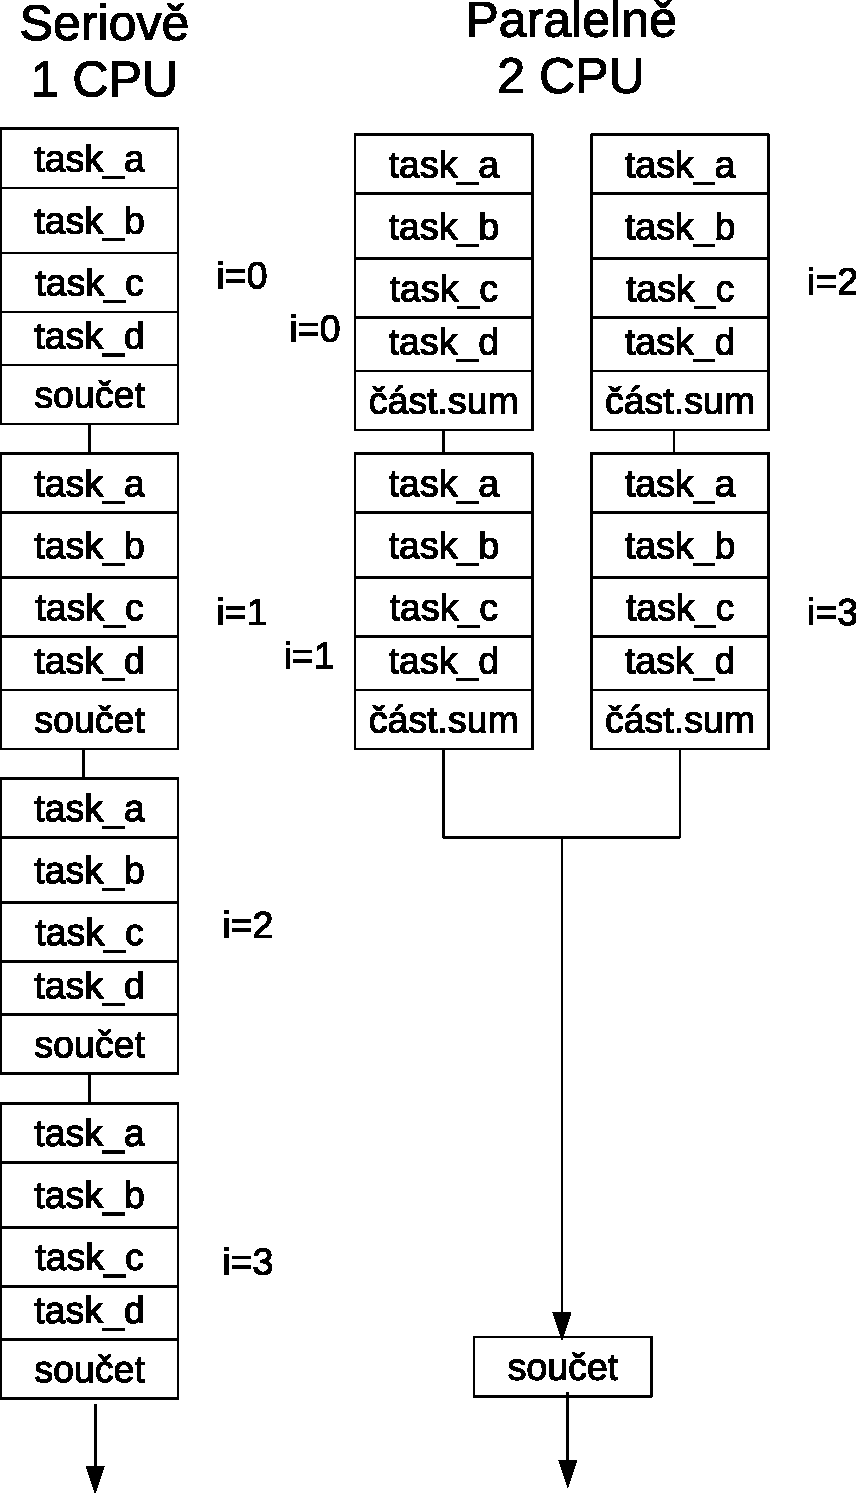
\includegraphics[scale=.6]{obr/serialvspara}
  \end{center}
  \caption{Porovnání sériového a paralelního přístupu}
  \label{obr:serialvspara}
\end{figure}

Během plánovací fáze paralelních programů je třeba vzít v úvahu některé stávající zákony. První zákon říká, že pokud program provádí nějaké \% časového kódu, který nelze provést paralelně, předpokládá se, že očekávaná rychlost z paralelizace bude v nejlepším zlepšení 1 / $y$. Zákon lze prokázat následovně. Předpokládejme, že $T_s$ představuje čas potřebný pro spuštění části kódu, kterou nelze paralelizovat, a $T_p$ představuje čas potřebný pro spuštění části kódu, který může mít prospěch z~paralelizace. Spuštěním programu s 1 procesorem je doba zpracování:

\begin{myequation}
\begin{aligned}
\label{vztah:serialcputimes}
T(1) = T_s + T_p
\end{aligned}
\end{myequation}

Když ale použijeme $N$ procesorů, tak je to méně:

\begin{myequation}
\begin{aligned}
\label{vztah:serialcputimes}
T(N) = T_s + T_p / N
\end{aligned}
\end{myequation}

Pokud řekneme, že $N$ jde do nekonečna, zrychlíme výpočet až $S = 1/y$. Tomuto zákonu se říká \emph{Amdahlův}.
         
\section{Datový paralelismus vs. úlohový paralelismus}

V paralelizaci jsou dva základní přístupy. Jedna instrukce a více dat (SIMD \ref{sec:simd}), které představuje datový paralelismus a Více instrukcí(jedna úloha) více dat (SPMD \ref{sec:spmd}) představující úlohový paralelismus.


\subsection{Datový paralelismus}


Takovým příkladem pro SIMD je sčítání vektorů. Všechny výpočetní jednotky provádějí stejnou instrukcí, každá však nad jiným indexem.


\subsection{Úlohový paralelismus}

Kdyby se však stejný postup místo na instrukce použil na celou úlohu, efektivita výpočtu by se zjevně snížila. Každá úloha by potřebovala jinak dlouhý časový úsek pro svou práci. 

\subsection{Load balancing}

Load balancing je technika, která dokáže využít plně možností víceprocesorového systému. Zde je implementována fronta procesů, ze které se systém postupně odebírá a přiděluje tak procesy volným jádrům.

\subsection{Pipeline}

\begin{figure}
  \begin{center}
    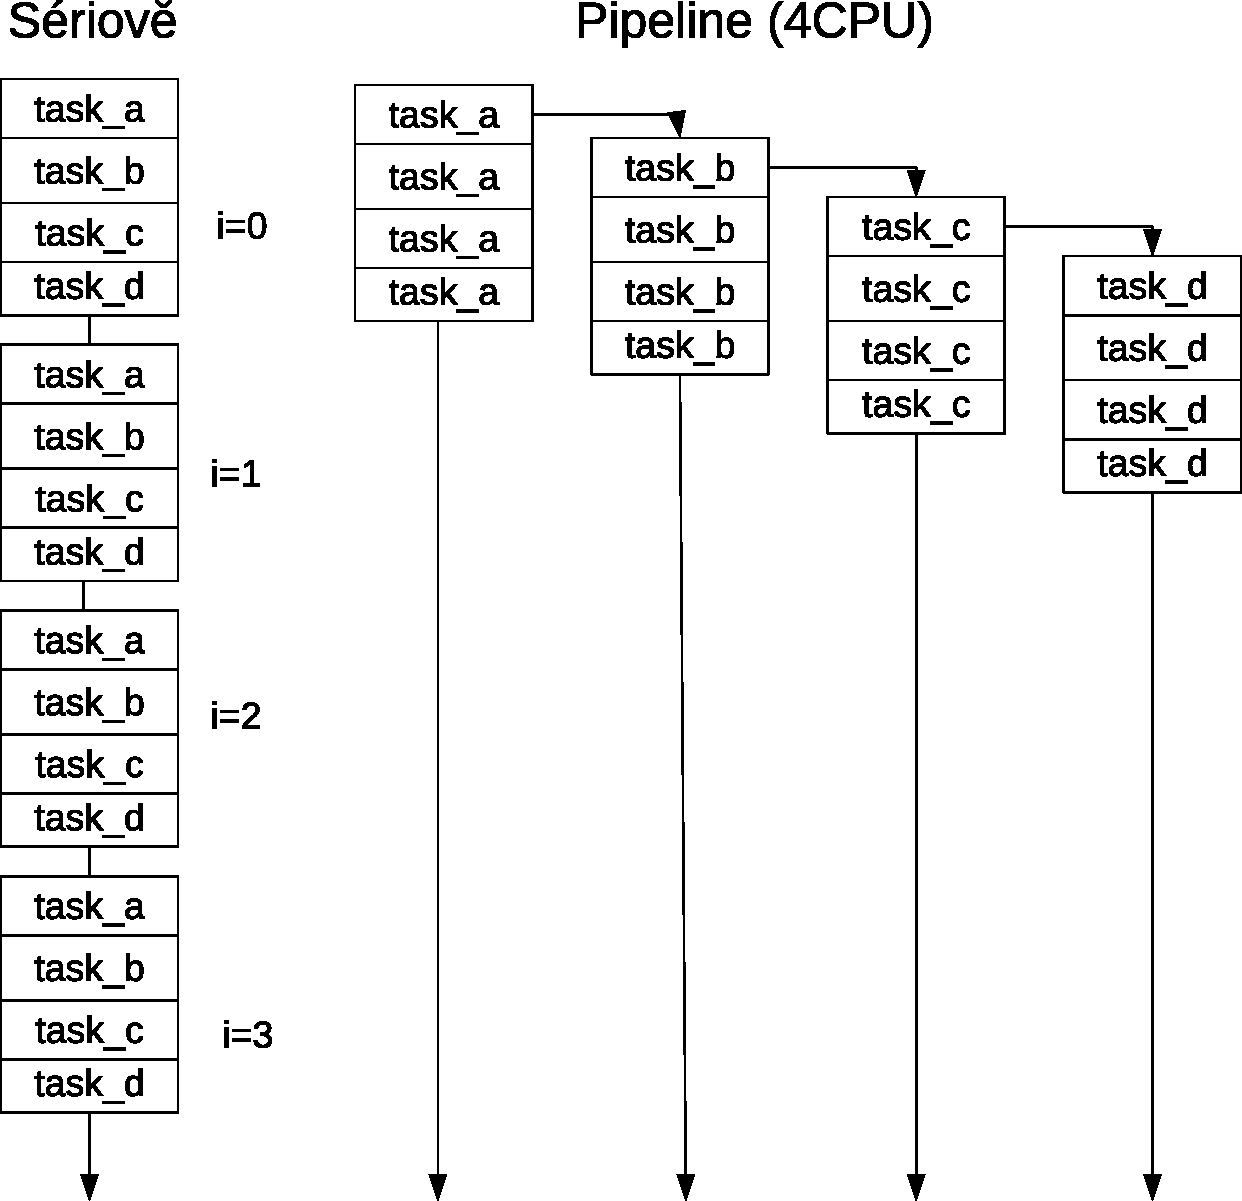
\includegraphics[scale=.6]{obr/pipeline}
  \end{center}
  \caption{Porovnání sériového přístupu a pipeline}
  \label{obr:serialvspipeline}
\end{figure}

Obrázek \ref{obr:serialvspipeline} ukazuje, že je možný ještě další přístup. Každý procesor je specializovaný na jednu určitou úlohu. Toto schema se s výhodou využívá
například u zpracování videa či signálů. 
\chapter{Program SoundAnalyzer}
\label{kap:programsoundanalyzer}

\section{Koncepce programu}

\emph{SoundAnalyzer} je grafická aplikace pro sledování signálu a jeho kmitočtové charakteristiky v reálném čase. Vytvořil jsem ji pro demonstrování, ale hlavně vyzkoušení pararelizovaného \emph{Goertzelova algoritmu}. Umí zobrazovat vstup z mikrofonu, výstup počítače (monitor výstupu) a také přehrávat zvukový soubor (formát \emph{wav}), nebo získaná data jako zvukový soubor uložit. Umí také provést jednorázový výpočet spektra ze souboru \emph{matlabu} a uložit jej též ve formátu \emph{matlabu}. Má velké možnosti konfigurace pro každý funkční blok (recorder, Goertzelův algoritmus, obecná nastavení).
Ačkoli je v této práci poskytnuta verze pouze pro linux, je program po úpravách multiplatformní.

\section{Použité knihovny}

Grafické uživatelské rozhraní je napsáno v jazyce \emph{QML} a knihovně \emph{Qt}. Tím je dosažena určitá multiplatformnost. Další důvod pro zvolení knihovny \emph{Qt} jsou mé zkušenosti s touto knihovnou a licenční politika.


Pro přehrávání a záznam zvuku ze zařízení je použita knihovna \emph{OpenAL}. Odkazy na funkce z ní jsou výhradně v bloku \emph{recorder}.


Pro zobrazení signálu je použita knihovna \emph{OpenGL}. Její funkční volání je použito výhradně v bloku \emph{barGraphRenderer}.

Vlastní výpočet využívá knihovnu \emph{OpenCL}, které je jako jediná proprietární, ale pro program šířený v rámci \emph{GNU GPLv2} je možné je použít. Jediné použití
\emph{OpenCL} funkcí je v bloku \emph{OpenCLGoertzel}.

Všechny bloku programu jsou pak napsány a pospojovány standardní knihovnou jazyka \emph{C++}. Funkce jazyka \emph{C} nejsou nikde v programu použity.

Více o použitých knihovnách najdete v kapitole \ref{kap:libraries}.

\section{Blokové schéma}
\label{sec:sablockscheme}

Zaměřme se nyní na obrázek \ref{obr:blockscheme}. Vidíme na něm blokové schéma programu \emph{Sound Analyzer}. Nyní proberu jednotlivé části podrobněji.

\begin{figure}
  \begin{center}
    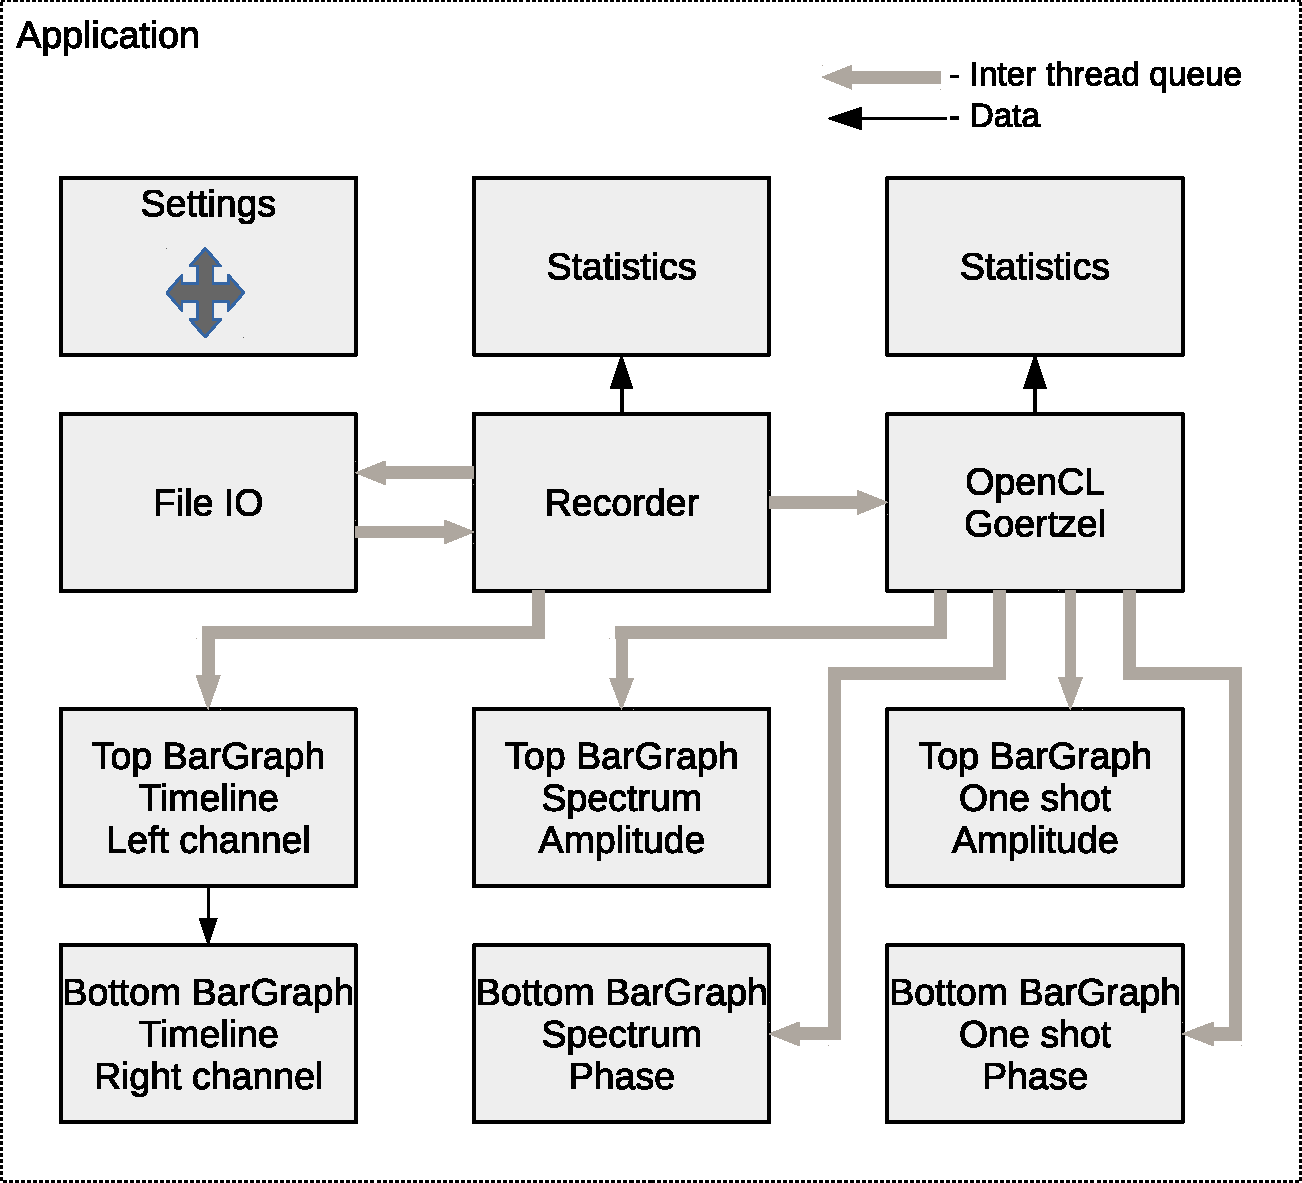
\includegraphics[scale=.7]{obr/SoundAnalyzeBlock}
  \end{center}
  \caption{Blokové schéma programu Sound Analyzer}
  \label{obr:blockscheme}
\end{figure}

\subsection{Inter thread queue}

Aplikace jako tato, která funguje jako přehrávač, záznamník, kreslí do okna
grafy, musí být nutně vícevláknová. Už jen proto, že závisí na spoustě
hardwaru a služeb současně a synchronizace mezi nimi je téměř nemožná.
Procesor totiž střídá vlákna po cca 10ms a pokud by se něco zdrželo ve
vymezeném čase pro hlavní vlákno, docházelo by zcela jistě k trhání a zpomalení
celé aplikace. Tato aplikace má tedy několik téměř samostatných funkcí, každá běžící ve svém vlákně. Problém souběhu řeší tato \emph{mezivláknová fronta}.

Blok \emph{mezivláknová fronta} tedy realizuje frontu opatřenou zámky. Současně poskytuje
zásobu segmentů, které může první vlákno naalokovat, zapsat do nich data a~zařadit do fronty. Druhé vlákno pak segment vyjme z fronty a vrátí. První vlákno nad to ještě může označit segment za poslední a když je přečten, další přečtené segmenty jsou již vždy \emph{nullptr}. Pro účely ladění se kontroluje, zda segment zařazený do fronty a vrácený segment, byly vydány touto frontou. Typická velikost zásoby segmentů je spočítána na cca 1 sekundu vzorků, minimálně však na 10 segmentů.

\subsection{\emph{OpenCL} Goertzel}

\emph{OpenCLGoertzel} je stěžejní komponenta celé aplikace. Vychází ze vztahu \ref{vztah:maticovygoertzelfinal}. Než ale začne samotný výpočet, je třeba spočítat matice $A$ a $D$. Matice $A$ je jednoduchá. Ale i zde lze provést dvě optimalizace. Protože budeme počítat s typem \emph{float -- 32 bitů}, lze očekávat možné nepřesnosti  dané malým počtem bitů. Jedno řešení je tedy jasné -- počítat konstanty v datovém typu \emph{double -- 64 bitů} a převést jen před vlastním zapsáním do grafické karty. Další operace jsou výpočty matice $A^k$, kde se na $k$ díváme jako
na binární číslo.

\begin{myequation}
\begin{aligned}
\label{vztah:rozkladak}
k = \dots k_3 . 2^3 + k_2 . 2^2 + k_1 . 2^1 + k_0 . 2^0 \\
A^k = \dots k_3((AA)(AA))((AA)(AA))  k_2(AA)(AA)  k_1 AA  k_0 A
\end{aligned}
\end{myequation}

tak počítám násobení matice nejvýše 6krát a nikoli 15krát jako kdybych počítal
prostým cyklem. Pokud mám různé mocniny $A$, snadno určím matici $D$.

Pokud bychom řekli, že sčítání mezivýsledků a počítání jednoho mezivýsledku dle vzorce \ref{vztah:maticovygoertzelfinal} trvá stejně dlouho, (jsou tam stejné matematické operace) dojdeme k~závěru, že optimální by bylo rozdělit výpočet série $N$ vzorků na
$N_M$.$N_L$ operací, kde $N_M$ a $N_L$ jsou stejné (přibližně odmocniny z $N$). Takto také tato komponenta počítá kolik cyklů ($L$) a kolik jader ($M$) bude použito pro výpočet. Já jsem v programu \emph{Sound Analyzer} ze začátku skutečně proměnné $L$ a a $M$ zavedl. Nyní se to již zdá být zbytečné, nicméně je to v programu stále, protože se ukázalo, že předpoklad ze začátku tohoto odstavce není úplně splněn a možná bude lepší jiný  algoritmus pro stanovení $L$ a $M$. Protože je možné doplnit řadu vzorků nulami, aniž by se ovlivnil výpočet, udělám to a zajistím si tak, že programy jader budou jednodušší, protože všechna jádra budou počítat stejný počet cyklů. Nakonec ani není třeba řešit, pokud by odmocnina z $N$ bylo iracionální číslo, prostě proměnné $L$ a $M$ zaokrouhlím nahoru. Ještě dodejme, že nuly se musí přidat před vzorky signálu, nikoli za něj.


Tato komponenta umí počítat nejen ze vzorků čerstvě přišlých z \emph{mezivláknové fronty}, ale i několika až $16386$ vzorků předchozích. Je tak možno získat větší přesnost, ale za cenu toho, že počítáme z delšího intervalu a výsledky tak nemusejí odpovídat okamžité realitě.


Na závěr sekce se zmíním o velikosti vektorů, se kterými lze počítat v knihovně \emph{OpenCL}. V dokumentaci \emph{OpenCL} je uvedena maximální velikost $16$ s tím, že je implementačně závislá a program si musí zjistit skutečnou velikost vektoru.
V případě mého grafického čipu \emph{AMD 7850} je to hodnota $8$. Ovšem já potřebuji složky vektoru sečíst a funkce, která to provádí, má podle dokumentace další omezení -- na velikost $4$. Nakonec tedy počítám s velikostí $4$. \emph{OpenCL} neumožňuje maticové operace.

Vlastní \emph{jádro}\ref{sec:kernel} je velmi jednoduché:

\begin{Verbatim} 

__kernel void main(
    __constant float*   streams,   //vstupní segment signálu
    __constant float*   D1,        //horní řádek matice D
    __constant float*   D2,        //dolní řádek matice D
    unsigned int        Channels,  //počet kanálů
    unsigned int        K,         //délka vektoru OpenCL, konstanta 4
    unsigned int        L,         //počet cyklů, respektive délka vektoru
                                   // se kterým pracujeme / 4
    unsigned int        M,         //počet jader spuštěných nad algoritmem
                                   // pro jeden kmitočet, jeden kanál		                               
    unsigned int        Length,    //délka segmentu
    __global float2*    outStreams //výtupní vektor
)
{
    unsigned int indexFrequency = get_global_id(0);
    unsigned int indexChannel = get_global_id(1);
    unsigned int indexItem = get_global_id(2);
    unsigned int i;
    float2 acc={0.0,0.0};
    __constant float4* data = (__constant float4*)&streams[indexChannel 
    		* Length + indexItem * L * K];
    __constant float4* mxD1 = (__constant float4*)&D1[indexFrequency 
    		* L * K];
    __constant float4* mxD2 = (__constant float4*)&D2[indexFrequency 
    		* L * K];
    for(i=0;i<L;i++)
    {
        acc.x = acc.x + dot(data[i] , mxD1[i]);
        acc.y = acc.y + dot(data[i] , mxD2[i]);
    } 
    outStreams[indexFrequency * Channels * M + indexChannel * M 
    		+ indexItem] = acc;
}
\end{Verbatim}

Funkci, jež má modifikátor \emph{\_\_kernel} \ref{sec:kernel} umíme jako jedinou spustit z hlavního programu a říkáme jí \emph{jádro}. Naše funkce má 9 parametrů, které mají před svými jmény modifikátory specifikující, ve které paměťové třídě se proměnná nachází. Více o těchto paměťových třídách najdete v kapitole \ref{kap:opencl}. Jak je vidět, program pouze realizuje cyklus:

\begin{myequation}
\begin{aligned}
\label{vztah:mojevariacestavw0_1}
outStreams[i_c][n] = \\
( \sum_{n=0}^{L-1} streams[i_c][n] . D_1[i_f][n] , \sum_{n=0}^{L-1} streams[i_c][n] . D_2[i_f][n] ),
\end{aligned}
\end{myequation}

kde $stream$ je blok vstupního signálu a $D_1[kmitočet],D_2[kmitočet]$ jsou přepočítané řádky matice $D$. Index kmitočtu je pak $i_f$ a index kanálu je $i_c$.


\subsection{Recorder}

\emph{Recorder} plní mezivláknovou frontu segmenty pro výpočet. Načítá je ze vstupního zařízení. Implicitní je určitě mikrofon, dále je možnost vybrat monitor výstupu, tedy provádět výpočet spektra nad signálem poskytovaným jinou aplikací. Volitelně může navíc ještě segmenty zkopírovat k zapsání do souboru komponentou popsanou níže.

Druhý režim \emph{recorderu} je přehrávání. Segmenty pořízené komponentou \emph{FileIO} jsou přehrány na standardním výstupu a zkopírovány do fronty pro výpočet spektra. Tím že jsou do této fronty kopírovány právě v okamžiku po jejich přehrání, je zajištěno časování.

Pokud je zvolen monitor standardního výstupu, nebo monitor HDMI výstupu, je signál zkreslen. Domnívám se, že je to ochrana proti kopírování. Záznam zvuku z~těchto monitorů totiž není zatížen ani minimálním šumem.

\subsection{File IO}

Souborové operace v programu \emph{Sound Analyzer} jsou načítání zvukového souboru ve formátu \emph{wav} do \emph{mezivláknové fronty} a samozřejmě i směrem z \emph{mezivláknové fronty} do souboru. V případě, že služby souborového systému jsou pomalejší než přísun segmentů,
jsou ve výsledném \emph{wav} souboru nespojitosti v tom smyslu, že je soubor je validní, dá se přehrát, ale jeho obsah je nespojitý.  Je také vypisováno hlášení na konzoli.
V případě, že souborový systém není schopen dodat dostatek dat pro přehrávání, mezivláknová fronta je prázdná a přehrávání je přerušované. I zde je vypisováno varovné hlášení na konzoli.


\subsection{Stats}

Komponenta statistiky je velmi jednoduchá. Má jen frontu hodnot a vždy zná jejich součet. Umí tak poskytnout kmitočet obnovování, vzorkovací kmitočet a  průměrný čas výpočtu spektra. Jednou za 0,5s vrací příznak, že komponenta, která statistiku vlastní, může zobrazit své data v uživatelském prostředí.

\subsection{Settings}


Nastavení je malá množina párů hodnota-klíč, sloužící k uchování nastavení. Její výhoda je přístup jak z \emph{C++}, tak z jazyka \emph{QML}. Po skončení aplikace se její obsah uloží do souboru a po startu je načten zpět.

\subsection{Application}

Aplikace všechny výše uvedené komponenty spojuje. Komponenty v \emph{Sound Analyzeru} jsou striktně odděleny a pokud spolu potřebují komunikovat nebo něco zobrazit, využívají funkce komponenty aplikace. Aplikace je jediná komponenta svázaná s grafickou knihovnou \emph{Qt}. Je ještě jedna funkce, kterou aplikace má. Při zapnutí nastaví všechny komponenty podle nastavení v komponentě settings a při změně pohledu mění propojení mezivláknových front.

\section{Licence}

Všechny použité knihovny jsou šířeny, nebo podporují \emph{GNU licenci}, takže i má práce musí být šířena pod licencí \emph{GNU GPLv2}.
\chapter{Knihovny použité při sestavování programu Sound Analyzer}
\label{kap:libraries}

V této kapitole vám přiblížím knihovny použité na projektu \emph{Sound Analyzer}.
Základem všech je ovšem stadardní knihovna jayka \emph{C++}.

\section{Knihovna openCL}
\label{kap:opencl}

Tato kapitola je výtahem z dokumentace k openCL (\cite{opencl}).
Úplnou dokumentaci lze najít \url{kronos.org}.

\subsection{OpenCL framework}

OpenCL \emph{framework} obsahuje tři hlavní části:

\begin{itemize}
\item OpenCL platformní vrstva -- dovoluje \emph{hostiteli} zjišťovat možnosti \emph{zařízení}, a~vytváří \emph{kontext}.
\item OpenCL runtime -- všechny operace manipulující s~kontextem.
\item Překladač openCL -- vytváří spustitelné objekty obsahující \emph{jádra}. Vychází z  ISO C99.
\end{itemize}

\subsection{Architektura openCL}

OpenCL je průmyslový standard pro programování heterogenních skupin CPU, GPU a~dalších zařízení organizovaných do jedné platformy. Je to více než jen jazyk.
Je to celý framework  který obsahuje programovací jazyk, API,
knihovny a~runtime systém pro podporu vývoje. OpenCL poskytuje nízkoúrovňovou
abstrakci hardware plus framework.
\\
V dalších kapitolách blíže popíši následující modely:
\begin{itemize}
\item Model platformy.
\item Model paměťový.
\item Model prováděcí.
\item Model programovací.
\end{itemize}

\subsection{Diagram tříd}

Obrázek (viz obr. \ref{obr:openclclassdiagram}) popisuje specifikaci openCL jako UML diagram tříd.
Jsou na~něm znázorněny jen základní třídy, nikoli jejich atributy.

\begin{figure}
  \begin{center}
    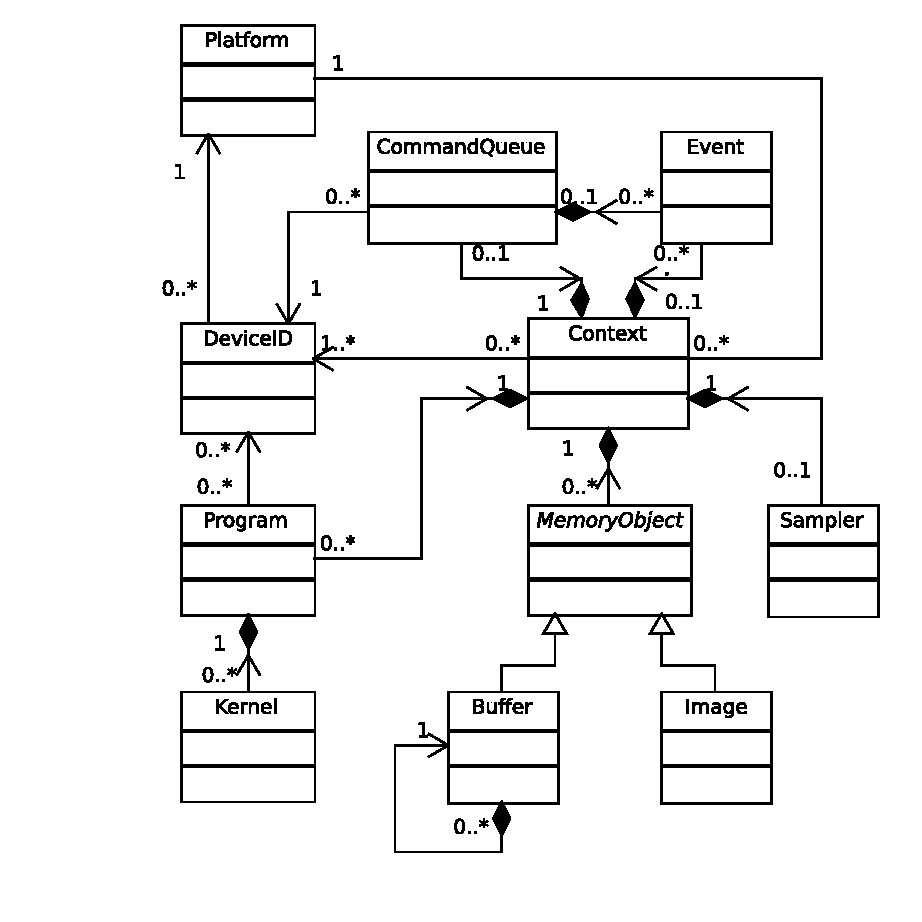
\includegraphics[scale=1]{obr/ClassDiagram}
  \end{center}
  \caption{UML Diagram tříd}
  \label{obr:openclclassdiagram}
\end{figure}

\subsection{Model platformy}

Model se sestává z \emph{hostitele}  připojeného k jednomu nebo více
openCL \emph{zařízením} . Toto  \emph{zařízení} je dále děleno
na~jednu nebo více \emph{výpočetních jednotek}  a~tyto
\emph{výpočetní jednotky} jsou dále děleny na~jednu nebo více \emph{zpracujících
jednotek} .

OpenCL \emph{aplikace}  běží na~\emph{hostiteli} 
OpenCL \emph{aplikace} posílá \emph{příkazy}  z \emph{hostitele}
ke zpracování výpočtů do \emph{zpracujících jednotek} 
v rámci \emph{zařízení}. \emph{Zpracující jednotky} v~rámci \emph{výpočetní jednotky}  provádějí jednu  sadu instrukcí jako \emph{SIMD} 
 jednotky, nebo jako \emph{SPMD}  jednotky, kde každá
\emph{zpracující jednotka} má svůj čítač instrukcí.

\subsubsection{Podpora různých verzí}

OpenCL je navrženo s~podporou více \emph{zařízení} s~různými možnostmi společně provozovanými pod jedním \emph{hostitelem}. To ovšem znamená, že každé zařízení může splňovat jinou verzi knihovny openCL. Máme tedy verzi runtime prostředí a~zvlášť verzi u~každého \emph{zařízení}. Dále každé \emph{zařízení} může podporovat svou vlastní verzi
jazyka openCL~C.


\subsection{Prováděcí model}

Když je \emph{jádro} pověřeno \emph{hostitelem} k provedení, je třeba definovat indexový prostor. Instance \emph{jádra}  se nazývá \emph{pracovní položka}  a~je definována bodem v~indexovém prostoru, který definuje \emph{globální ID}  pro tuto \emph{pracovní položku}. Pracovní položka je svázánu s jedním, konkrétním jádrem výpočetního zařízení.\emph{Pracovní položky}
jsou organizovány v~ \emph{pracovních skupinách} .
\emph{Pracovní skupiny} mají unikání ID \emph{pracovní skupiny}. \emph{Pracovní položky} můžeme v~indexovém prostoru identifikovat stejným způsobem, Také mají své \emph{globální ID}. Mimo to je ale můžeme identifikovat dvojicí \emph{globální ID} \emph{pracovní skupiny} a~\emph{lokálním ID} (v rámci této \emph{pracovní skupiny}).
\\
Indexový prostor, který je definován knihovnou openCL, je $N$-rozměrná pole. Nazývají se \emph{NDRange}. $N$ může být jedna, dvě nebo tři. To znamená, že i indexy jsou $N$-prvkové. Položky indexu začínají vždy od nuly.
\\
Index tedy definuje určitou \emph{pracovní skupinu} v~rámci \emph{výpočetní jednotky}. Stejným způsobem je také definován index \emph{pracovní položky} v~rámci \emph{pracovní skupiny}.

\subsubsection{Kontext a~fronty příkazů}	

\emph{Kontext}  vytváří a~spravuje \emph{hostitel} prostřednicvím funkčních volání openCL API. \emph{Hostitel} v~\emph{kontextu} vytvoří zejména \emph{frontu příkazů} , aby mohl zařízení ovládat. Do těchto \emph{front příkazů} zapisuje \emph{příkazy} k provedení. Mezi tyto \emph{příkazy} patří:

\begin{itemize}
\item Příkazy k provádění jádra.
\item Příkazy pro práci s~pamětí.
\item Synchronizační příkazy.
\end{itemize}


V jednom \emph{kontextu} může být více \emph{front příkazů} které jsou prováděny nezávisle na~sobě.


\subsection{Paměťový model}

\emph{Pracovní položky} rozlišují čtyři druhy pamětí:

\begin{itemize}
\item Globální paměť.
\item Paměť konstant.
\item Lokální paměť.
\item Soukromá paměť.
\end{itemize}


\begin{table}[htbp]
\centering
 
\begin{tabular}{|c||c|c|c|c|}
\hline
Přístup z& \bfseries Global & \bfseries Constant & \bfseries Local & \bfseries Private \\
\hline
\hline
\multirow{5}{*}{\bfseries Hosta}  & Dynamická & Dynamická & Dynamická & Bez\\
& alokace & alokace & alokace & alokace\\
& & & &\\
& Přístup pro & Přístup pro & Není & Není\\
& čtení / zápis & čtení / zápis & přístup & přístup\\
\hline
\multirow{5}{*}{\bfseries Jádra}  & Není & Statická & Statická & Statická\\
& alokace & alokace & alokace & alokace\\
& & & &\\
& Přístup pro & Přístup pro & Přístup pro & Přístup pro\\
& čtení / zápis & jen čtení & čtení / zápis & čtení / zápis\\
\hline
\end{tabular}
\caption{Typy pamětí v~openCL}
\label{tab:typypameti} 
\end{table}

\emph{Aplikace} běžící na~\emph{hostiteli} vytváří \emph{paměťové objekty} v~{globální paměti}.


Paměť \emph{hostitele} a~\emph{zařízení} jsou na~sobě nezávislé. Nicméně je potřeba aby \emph{zařízení}
a~\emph{hostitel} spolu nějakým způsobem komunikovaly.
Toho je docíleno kopírováním paměti nebo jejím sdílením. Kopírování může býti jak blokující,
tak neblokující. Blokující nebo neblokující může být
rovněž mapování paměti. \emph{Aplikace} většinou
mapuje paměť na~nezbytně nutnou dobu a~když jsou všechny operace čtení a~zápisu dokončeny, opět
paměť odmapuje.

\subsection{Programovací model}

OpenCL nabízí dva programovací modely, respektive dva základní přístupy. \textbf{Datově paralelní model} a~\textbf{úlohově paralelní model}.

\subsubsection{Datově paralelní model}

V datově paralelním programovacím modelu provádějí všechny \emph{pracovní položky} v~rámci \emph{pracovní skupiny} současně jednu sadu instrukcí. Model je rozdělen na~dvě kategorie.
U \textbf{explicitní} definuje aplikace, jak bude \emph{pracovní skupina} rozdělena na~\emph{pracovní položky}. U \textbf{implicitní} aplikace pouze definuje, kolik pracovních položek chce použít a~rozdělení \emph{pracovní skupiny} na~\emph{pracovní položky} nechá na~knihovně openCL.

\subsubsection{Úlohově paralelní model} 

V úlohově paralelním modelu je každé \emph{jádro}\ref{sec:kernel} vykonáváno zcela nezávisle na~jiných. Znamená to, že je prováděno v~\emph{pracovní skupině}, která má jednu jedinou \emph{pracovní položku}. V~tomto modelu je zdůrazněna paralelnost:

\begin{itemize}
\item používáním vektorových datových typů.
\item řízením více úloh.
\end{itemize}

\subsubsection{Synchronizace}

\emph{Pracovní položky} položky mohou být synchronizovány mezi sebou využitím \emph{bariér}. Pro synchronizaci \emph{pracovních skupin} mezi sebou, žádný takový mechanismus neexistuje.

\emph{Příkazy} mají také možnost používat \emph{bariéry}. Tyto \emph{bariéry} zajistí, že všechny příkazy zařazené před touto \emph{bariérou} ve \emph{frontě příkazů}, budou provedeny dříve, než se začne s~prováděním dalších \emph{příkazů}.

Všechny \emph{příkazy} \emph{hostitele}, které  vkládají \emph{příkazy} do \emph{fronty příkazů}, vracejí objekt \textbf{události}. Další \emph{příkaz} ve \emph{frontě příkazů} může na~tuto událost čekat.

\subsection{Paměťové objekty}

Jsou dvě kategorie \emph{paměťových objektů}: \emph{obrázky}  a~\emph{buffery} .
\emph{Buffer} je řada objektů nějakého typu a~můžeme k nim přistupovat pomocí rukojeti (handle \ref{sec:handle}). Naproti tomu je struktura \emph{obrázku} skryta a~k \emph{obrázku} můžeme přistupovat pouze pomocí speciálních funkcí jádra. \emph{Obrázek} nemusí mít stejný formát u \emph{hostitele} a~uvnitř \emph{jádra}.




\section{OpenGL}

\subsection{Historie OpenGL}

Do devadesátých let minulého století panovalo všeobecné nadšení
z výpočetního výkonu počítačů dovolujícího kreslit 3D grafiku. Byla řada výrobců hardware. Bohužel byla i velká řada výrobců vytvářejících vlastní grafické knihovny a ovladače. Žádný tak neuměl zacházet s jakýmkoli hardwarem a měl tedy jen malou omezenou množinu aplikací.
Vznikla tak nutnost unifikace.


V další dekádě byla špičkou v grafice společnost \emph{SGI}. Vyvinula svůj standard \emph{IrisGL}. Jeho nevýhodou bylo začlenění funkcí pro \emph{X11} a použití patentovaných algoritmů. Proto začali ostatní výrobci pracovat na rozhraní od \emph{IrisGL} odvozeném a~nazvali jej \emph{OpenGL}.


V roce 1992 bylo pro účely správy \emph{OpenGL} vytvořeno konsorcium
\emph{OpenGL} ARB.	V roce 2006 byla \emph{OpenGL} předána konsorciu \emph{Kronos Group}.

\subsection{Vykreslovací řetězec}

\emph{OpenGL} popíšu jen lehkým úvodem. Začnu s popisem vykreslovacího řetězce, jak jej uvedli Procházka, Koubek a a Andrýsková v \cite{mendelu}. V současných verzích \emph{OpenGL} je ještě složitější, takto odpovídá verzi \emph{OpenGL}
2.0.

\begin{figure}[hbt]
  \begin{center}
    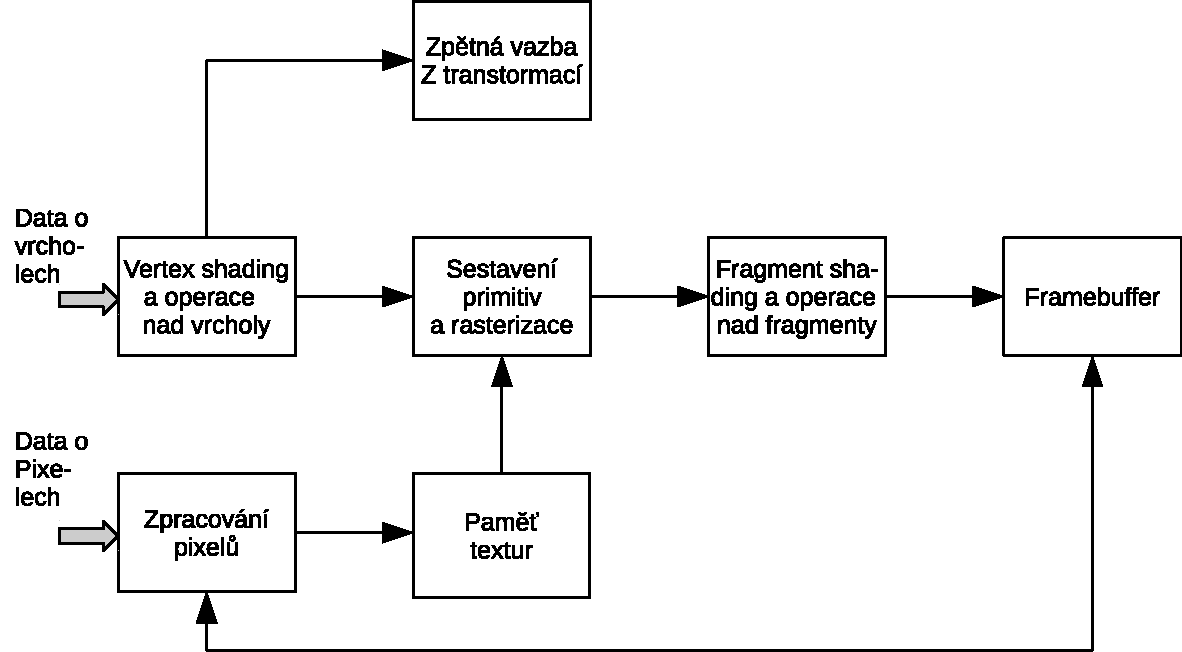
\includegraphics[scale=.6]{obr/opengl}
  \end{center}
  \caption{\emph{OpenGL} vykreslovací řetězec}
  \label{obr:openclglassdiagram}
\end{figure}

\subsubsection{Framebuffer}

Framebuffer je paměť jejíž obraz je bude zobrazen. Framebuffery jsou většinou dva nebo více, jeden se synchronně posílá na zobrazovací zařízení, ve druhém
je tvořen následující snímek.

\subsubsection{Zpracování pixelů}

Grafický subsystém, jakožto rasterové zařízení umožňuje práci s rasterovými daty. V postatě je schopen je jen zapsat/vyčíst framebufferu a zapsat do paměti textur.

\subsubsection{Zpracování vrcholů}

Vrchol (vertex) není jen bod v prostoru. V \emph{OpenGL} má vertex kromě své pozice řadu dalších uživatelských vlastností, které lze z programu nastavit a také je při zpracování vrcholu využít. Dříve byla tato jednotka fixní, grafický čip prováděl vždy stejnou operaci nad vrcholy. Nyní, od \emph{OpenGL} 2.0, je vykreslovací řetězec programovatelný a tato jednotka může vykonávat s vrcholem jakoukoli operaci pomocí programu v jazyce \emph{GLSL}. Lze tak realizovat základní operace s vrcholem, jako otočení, změna měřítka, posunutí, ale i třeba efekty jako jsou vlny na hladině, efekt lomení paprsku na hladině a podobně.

\subsubsection{Sestavení primitiv a rasterizace}

Když předchozí jednotka stanovila již definitivní souřadnice ploch, je třeba z každé jednotlivé plochy
získat množinu bodů, které odpovídají pixelům na zobrazovacím zařízení, fragmentům.

\subsubsection{Fragment shading a operace nad fragmenty}

Stejně jako vertex není jen bod v prostoru, tak i fragment obsahuje více informací než jen polohu a barvu. Tato jednotka je od \emph{OpenGL} 2.0 programovatelná v jazyce \emph{GLSL} a umožňuje nanášet textury, vybarvovat pixel podle jeho polohy (barevný přechod), některé efekty se světlem, míchání barev a podobně.

\section{OpenAL}

\emph{OpenAL} (\uv{Open Audio Library}) je softwarový interface k
audio hardwaru. Interface poskytuje několik funkcí, kterými
program modeluje objekty generující ve 3D prostoru a samozřejmě zajišťuje mixování všech zvuků od všech objektů.
Nepodporuje přímo stereo ozvučení, naproti tomu prostě propočítá \emph{streamy} pro potřebný počet kanálů. Nabízí také 
zpracování efektů jako je Doplerův jev, odrazy, překážky,
vysílání a 	dozvuky.

\emph{OpenAL} je implementováno pro většinu platforem.


\subsection{Historie \emph{OpenAL}}

\emph{OpenAL} bylo původně vyvinuto společností \emph{Loki Software} jako
doplněk ke knihovně \emph{OpenGL} asi okolo roku 1998. Dále jej udržuje Creative Technology, která jako první uvolnila hardwarově akcelerovanou \emph{OpenAL}.


\subsection{Stručný popis}

\begin{figure}[hbt]
  \begin{center}
    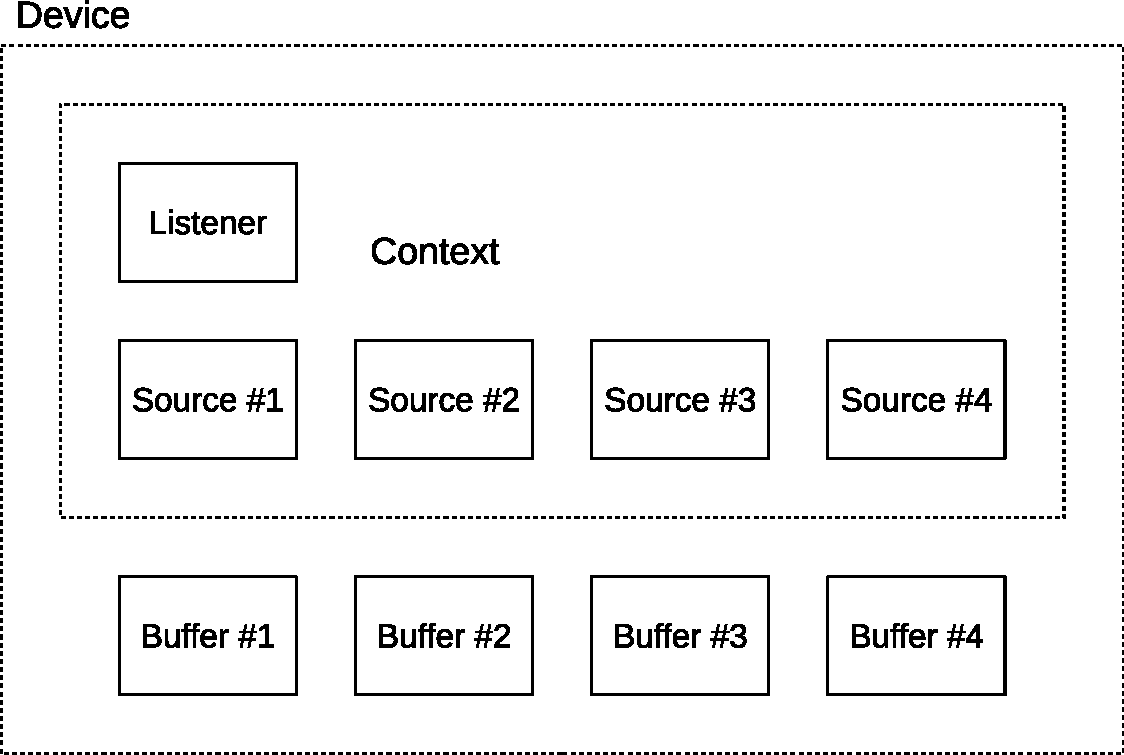
\includegraphics[scale=.6]{obr/openal}
  \end{center}
  \caption{\emph{OpenAL} struktura API}
  \label{obr:openclalassdiagram}
\end{figure}

V \emph{OpenAL} je jeden Posluchač (Listener) který reprezentuje výstup.
Ten je tvořen jedním nebo mnoha, klidně stovkami zvuků od Zdrojů
(Sources). Každý zdroje má kromě zaznamenaného zvuku také přiřazen vzorkovací kmitočet, polohu a vektor rychlosti (pro výpočet Dopplerova efektu). Zdroj přehrává data z jednoho nebo fronty několika bufferů.
\section{\emph{Qt}}

\emph{Qt} je multiplatformní framework. Je definován snad na všechny desktopové i mobilní operační systémy. Je vydáván ve dvou licencích. \emph{LGPL} umožňuje volné šíření \emph{Qt}, ale neumožňuje statické linkování, jsou dostupné jen základní částni bez přídavných modulů, programátor musí dát návod jak vyměnit dynamicky linkované knihovny za novější, licence jeho produktu musí být také \emph{LGPL}. Výše uvedené nedostatky řeší licence proprietární.

\subsection{Historie}

Historie \emph{Qt} se začala datovat v roce 1990 v Norsku. V roce 1995 bylo první vydání firmou Trolltech. V roce 2005 bylo \emph{Qt} zcela přepracováno na verzi 4.0. V roce 2008 byl Trolltech koupen Nokií. V roce 2010 Nokia vydává Symbian, operační systém pro smartphony založený na \emph{Qt}. V roce 2012 byl představen jazyk \emph{QML} a \emph{Qt} 5.0. \emph{Qt} se stalo samostatnou společností v roce 2014.

\subsection{Koncept signál-slot}

V \emph{Qt} je alternativa k callback funkcím, je to koncept signál-slot. Když nastane nějaká
událost, je emitován signál. Slot je funkce , která je volána jako odezva na emitovaný signál. V \emph{Qt} je řada předdefinovaných signálů, ale lze jednoduše tvořit signály vlastní. 


Signály a sloty jsou typově bezpečné, čímž se míní skutečnost, že parametry, respektive typy a počet parametrů jsou u signálu i slotu stejné.


Je varianta, kde se signál a slot propojí jmény funkcí (string based), překlad jména funkce na volání skutečné funkce se provádí za běhu aplikace.


Signály a sloty jsou vláknově bezpečné, dokonce se ve vícevláknových aplikacích požívají pro mezivláknovou komunikaci.

\subsection{\emph{QML}}

Ve verzi 5 \emph{Qt} představilo jazyk \emph{QML}. Je to deklarativní jazyk, který popisuje layout
uživatelského rozhraní. Nad to obsluha událostí je nyní ve stejném \emph{QML} souboru v~jazyce javascript.
Celý kontroler se tak přesunul na novou platformu.

Přesto je stále možné tvořit ovládací prvky pro \emph{QML} v jazyce C++, volat z~\emph{C++}
\emph{javascriptové} funkce a volat z~\emph{javascriptových} funkcí \emph{C++} funkce.


Velkou novinkou je zavedení \emph{vlastností} (properties) objektů v \emph{QML}. Nastavení vlastnosti nemusí být jen konstanta, ale i složitější konstrukce v jazyce \emph{javascript}.
Pokud se jedna nebo více proměnných, na kterých \emph{vlastnost} závisí změní, dojde k~automatickému přepočítání a je stanovena nová hodnota proměnné-vlastnosti.


Úskalím tohoto konceptu je, že při neopatrném zacházení s vlastnostmi mohou vznikat cyklické závislosti, kde jedna \emph{vlastností} závisí na druhé, ale ta současně na první. Často nejsou tyto závislosti zřejmé.

Předchozí tzv. widgetové aplikace se nedají s tímto novým konceptem kombinovat. Je ale stále možné takovéto widgetové aplikace v \emph{Qt} 5 vytvářet.


Daní za \emph{QML} je nižší výkon aplikace a vysoké paměťové nároky. Výhodou má naopak být rychlost vývoje a aplikace \emph{javasriptu} je velmi stabilní i po chybě programátora.

\chapter{Měření přínosu využití grafického čipu}
\label{kap:measurement}

Aby bylo možno nějakým způsobem prověřit funkčnost programu, jsou do něj přidány některé měřící funkce.

\section{Počet využívaných jader}

První informace která je obecně zajímavá, je kolik jader \emph{GPU} potřebuji, kolik jich mám k dispozici a kolik jsem chopen jich reálně využít. Proto je na liště nástrojů programu \emph{Sound Analyzer} sedm údajů: Globální $N/C/M$, lokální $N/C/M$ a maximální počet jader současně spustitelných. Více o počtu jader najdete v manuálu, sekci \emph{Počet jader použitých při výpočtech} \ref{sec:nkernels}.

\section{Průměrná délka výpočtu za poslední dobu}

Program měří čas každého provedení výpočtu v mikrosekundách. Využívá přitom komponentu \emph{Stats}, které implementuje frontu 250 hodnot. Z těchto 250 hodnot je počítán aritmetický průměr.


\section{Metodika měření}

Abychom změřili uspořený čas \emph{CPU}, bylo by dobré nejdříve provést měření které nezatěžuje \emph{GPU}, tedy nějaký jednoduchý výpočet. Potom provedu měření zatížení všech jader, ale tak, aby globální počet jader se rovnal lokálnímu počtu jader, tedy jeden výpočetní cyklus. Jako třetí měření zatížím \emph{GPU} tak, abych maximálně využil paměť. Při velkých požadavcích \emph{OpenCL} jednoduše vrátí chybu.


Při všech těchto měřeních by bylo jistě zajímavé vědět, jak je zatížen počítač jako takový. Ideální na to je program \emph{mstats} z balíku \emph{sysstat}. Budu počítat zatížení procesoru za periodu 10s.


Ještě připomenu, že v programu \emph{Sound Analyzer} se délkou segmentu myslí délka, kterou \emph{recorder} načte ze vstupního zařízení. K se přičítá $overlap$ vzorků z předchozích segmentů.


\section{Použité počítače}

\subsection{PC1}

\begin{table}[htbp]
\centering
\caption{Parametry testovacího počítače}
\begin{tabular}{|l|l|}
\hline
Operační systém&Linux Mint 17.3 64bit\\
CPU model&AMD FX-8350\\
CPU jader&8\\
CPU kmitočet& 4000MHz\\
Paměť& 32GB\\
Chipset&AMD 990FX\\
GPU model&AMD Radeon HD7850\\
GPU paměť&2GB\\
GPU jader&1200\\
GPU kmitočet& 1000MHz\\
\hline 
\end{tabular}
\end{table}

\subsection{Notebook1}


\begin{table}[htbp]
\centering
\caption{Parametry testovacího notebooku}
\begin{tabular}{|l|l|}
\hline
Operační systém&Linux Mint 18.1 64bit\\
CPU model&Intel i7-4850HQ\\
CPU jader&4 (8 vláken)\\
CPU kmitočet& 2300MHz\\
Paměť& 16GB\\
Chipset&-\\
GPU model&NVidia GeForce GT 750M Mac edition / Intel IRIS 5200\\
GPU paměť&2GB / 128MB\\
GPU jader&384 /-\\
GPU kmitočet& 926MHz/-\\
\hline 
\end{tabular}
\end{table}

\subsection{Další podmínky měření}

$f_{vz} = 8000Hz$ \\
Na počítačích byl spuštěn pouze program \emph{Sound Analyzer} a terminál s programem \emph{mstats}.

\section{Naměřené hodnoty}

\subsection{PC1}

\begin{table}[htbp]
\centering
\caption{Naměžené hodnoty pro pro testovací počítač}
\begin{tabular}{|c|c|c|c|c|c|c|c|c|}
\hline
Kmit. & Segm. & Over- & Globální & Lokální & CPU & CPU & GPU & GPU\\
počet & délka & lap & NDRange & NDRange & doba & využití & doba & využití\\
$\left[ - \right]$ & $\left[ - \right]$ & $\left[ - \right]$ &$\left[ -/-/- \right]$ & $\left[ -/-/- \right]$ & $\left[ \mu s\right]$ & $\left[ \% \right]$ & $\left[ \mu s \right]$ & $\left[ \% \right]$\\
\hline
0&0&0&0/0/0&0/0/0&-&4,83&-&-\\
1&4&0&1/1/1&1/1/1&105&6,54&160&7,13\\
1&512&15872&1/1/64&1/1/64&230&5,3&410&5,0\\
16384&4&0&16384/1/1&1024/1/1&300&24,4&-&-\\
16384&512&15872&16384/1/64&16/1/64&61090&82,64&-&-\\
64&512&15872&64/1/64&16/1/64&690&5,25&-&-\\
64&512&15872&64/1/64&4/1/64&-&-&430&5,20\\
\hline
\end{tabular}
\end{table}

\subsection{PC1 - měření využití jader}


\begin{table}[htbp]
\centering
\label{tab:pc1mvj}
\caption{Naměřené hodnoty pro měření využití jader pro testovací počítač}
\begin{tabular}{|c|c|c|c|c|c|c|c|c|c|}
\hline
Lokální & \multicolumn{9}{c|}{Globální počet jader $\left[ \mu s\right]$}\\
počet & 1 & 2&4&8&16&32&64&128&256\\
jader & &&&&&&&& \\
$\left[ \mu s\right]$ &&&&&&&&&\\
\hline
1&154&-&-&-&-&-&-&-&-\\
2&154&154&-&-&-&-&-&-&-\\
4&154&154&154&-&-&-&-&-&-\\
8&155&155&155&155&-&-&-&-&-\\
16&155&155&155&155&155&-&-&-&-\\
32&156&156&156&156&156&156&-&-&-\\
64&157&157&157&157&157&157&157&-&-\\
128&157&157&157&157&157&157&157&157&-\\
256&158&158&158&158&158&158&158&158&158\\
\hline
\end{tabular}
\end{table}


\subsection{Notebook1}
\begin{table}[!h]
\centering
\caption{Naměžené hodnoty pro pro testovací notebook}
\begin{tabular}{|c|c|c|c|c|c|c|c|c|}
\hline
Kmit. & Segm. & Over- & Globální & Lokální & CPU & CPU & GPU & GPU\\
počet & délka & lap & NDRange & NDRange & doba & využití & doba & využití\\
$\left[ - \right]$ & $\left[ - \right]$ & $\left[ - \right]$ &$\left[ -/-/- \right]$ & $\left[ -/-/- \right]$ & $\left[ \mu s\right]$ & $\left[ \% \right]$ & $\left[ \mu s \right]$ & $\left[ \% \right]$\\
\hline
0&0&0&0/0/0&0/0/0&-&4,11&-&-\\
1&4&0&1/1/1&1/1/1&-&-&105&6,41\\
1&512&15872&1/1/64&1/1/64&-&-&610&4,50\\
16384&4&0&16384/1/1&1024/1/1&-&-&190&8,85\\
16384&512&15872&16384/1/64&16/1/64&-&-&161410&10,12\\
64&512&15872&64/1/64&16/1/64&-&-&1265&4,62\\
\hline
\end{tabular}
\end{table}

\section{Shrnutí}

Prvně je třeba vysvětlit nenaměřené hodnoty. U \emph{NVidie} vrátí inicializační funkce chybu vždy, když se pokusíme použít výpočet procesorem. U \emph{AMD} je nějaký limit na paměť okolo 4000 jader, po jeho překročení \emph{OpenCL} vrátí chybu \uv{Failed to execute kernel! (2) err=0xfffffffb}, což znamená \uv{Nemohu naalokovat paměť}.


Z prvních řádků obou měření je vidět, kolik času zabírá hlavní smyčka programu, která po cca 100ms překresluje okno. Lehce silnějším se zdá být procesor \emph{i7}.

Poté jsem spustil jedno jediné jádro a vidím, že požadavky na \emph{CPU} vzrostly asi dvojnásobně, protože počítáme cca 2000krát za jednu sekundu. Je též patrné, že
funkční volání, které spouští \emph{OpenCL}, trvá asi 105$\mu s$ na \emph{NVidii} a~160$\mu s$ na \emph{AMD}. Pod tyto časy už se zřejmě nepůjde dostat.

Pak se dá zkusit počítat jednu dlouhou řadu s 64 mezivýsledky, tedy s~využitím 64 jader. Jak patrno, potřebný výkon \emph{CPU} značně klesl, protože počítáme s~nižším obnovovacím kmitočtem, asi jen 15,6 Hz, oproti 2000Hz v případě předchozím. U~\emph{AMD} to zvedlo potřebu \emph{CPU} o pouhých 0,17\% a doba strávená výpočtem je větší asi jen čtyřnásobně. U \emph{NVidie} stoupla potřeba \emph{CPU} o 0,39\% a výpočet je delší méně než šestinásobně.


Ještě se podívejme na poslední řádky tabulek naměřených hodnot. Zde počítáme hodnoty pro 64 kmitočtů a 16384 vzorků dlouhé řady. Zatížení \emph{CPU} je pro oba grafické čipy minimálních 0,39\%. Grafický desktopový čip \emph{AMD} je ale výrazně rychlejší než mobilní \emph{NVidie}. Z předposledního řádku první tabulky je vidět, že počítání CPU je asi o polovinu pomalejší.


Nakonec jsem ještě změřil, jak moc pomáhá grafický čip procesoru. Měřil jsem tak, že jsem upravil program \emph{SoundAnalyzer} na možnost ovlivnění počtu lokálních jader.
Zastavil jsem $1,2,4,8,16,32,64,128~a~256$ jader jako požadavek (globální) tak jako lokální. Výsledek je celkem překvapující a je v tabulce \ref{tab:pc1mvj}. Ať jsem nastavil jakýkoli počet jader, doba strávená výpočtem byla vždy $154~až~158 \mu s$, tedy jen lehce úměrná počtu spouštěných výpočetních jednotek. Knihovna \emph{OpenCL} tedy nebere parametr $lokální NDRange$ jako počet procesorů, které chceme použít, ale použije vždy veškeré možné. Čím více mezivýsledků sčítám, tím je provádění delší, ačkoliv ten rozdíl na 256ti výpočetních jednotkách byl pouze $4 \mu s$. Protože ale není možné spustit pouze jedno jádro, nejsem schopen s přesností porovnat pararelní a seriový přístup. Navíc doba provádění je tak malá, že ji lze jen těžko měřit prostředky PC. Navíc tato doba hodně kolísá díky tomu, že v počítači běží řada různých procesů. Přes to lze říci, že paralelizace se vyplatila. Výpočet 256krát delší zátěže trvá jen o~cca 0,25\% déle.


Závěrem sekce ještě uvedu srovnání počtu jader ve vztahu k předpokladům daných hardwarem. Ačkoli \emph{GPU AMD} má 1200 jader, \emph{OpenCL} nabízela k použití vždy jen 256 jader. Na proti tomu 384jádrová \emph{NVidia} nabízela k výpočtu vždy 1024 jader. Softwarové zpracování poskytovala pouze \emph{GPU AMD} a nabízela vždy 1024 jader.

\section{Závěr měření}

Z výsledků je patrné, že využití {GPU} ke zpracování signálu skutečně může výrazně odlehčit hlavnímu procesoru. Je ale třeba brát v úvahu několik předpokladů. Zatížení \emph{GPU} nesmí být nesmyslně malé. Je tu totiž velká režie s voláním \emph{OpenCL} funkcí a~jednoduše se to nemusí vyplatit. Zejména mám na mysli počítat v každé výpočetní jednotce dostatečně dlouhý blok signálu. Rozdělení segmentu signálu na bloky se tedy vyplatí jen u segmentů delších něž cca 2048 vzorků.


 Je to patrné z prvních řádků tabulek, kde přenesení výpočtu na\emph{CPU} výpočet výrazně urychluje.

Aplikace by také měla být vícevláknová s jedním vyhrazeným vláknem pro výpočet na \emph{GPU}, zejména pro případ realtimeové aplikace.

%% Vložení souboru 'text/reseni' s popisem reseni práce
%\chapter{Teoretická část studentské práce}

Teoretické zázemí studentské práce vhodně rozdělené do částí.

(Struktura navržená v~této šabloně je nehrubší možná, po konzultaci s~vedoucím je vhodné zvolit přiléhavější.)


%% Vložení souboru 'text/vysledky' s popisem vysledků práce
%\chapter{Výsledky studentské práce}

Praktická část a výsledky studenstké práce vhodně rozdělené do částí.


%% Vložení souboru 'text/zaver' se závěrem
%\chapter{Závěr}

V kapitole \uv{Možnosti paralelizace} (\ref{kap:moznostireseni}) jsou uvedeny tři hlavní směry, kterými by se měla diplomová práce ubírat. Prvně bylo ukázáno, že výpočet se dá za cenu mírného zesložitění rozdělit na více procesorových jednotek a 
následně mezivýsledky spojovat. Dále je v téže kapitole ukázáno, jak využít možnost maticových operací (\ref{kap:matrixoperations}), které nabízejí dnešní grafické čipy. Jako poslední směr je uvedena možnost počítání několika kmitočtů současně (\ref{kap:multifrequency}). V textu je několik otázek, na které lze odpovědět pouze provedením nějakého testu. Například, zda počítání s maticemi velikosti $4\cdot 4$ skutečně urychlí výpočet oproti popsané skalární variantě (\ref{kap:matrixoperations}). %Dalším testem je ověřit, zda je vhodné počítat součin dvou matic $4\cdot 4$ a následně %funkci $diag$, nebo součet dvou součinů matic $4\cdot 1$.
\chapter{Závěr}

V kapitole \uv{Možnosti paralelizace} (\ref{kap:moznostireseni}) bylo ukázáno, že výpočet se dá za cenu mírného zesložitění rozdělit na více procesorových jednotek a 
následně mezivýsledky spojovat. Byly vybrány knihovny pro vývoj aplikace. Po bližším zkoumání několika možných knihoven byly použity knihovny \emph{OpenCL}, \emph{OpenAL}, \emph{OpenGL}, \emph{Standardní C++} a \emph{Qt}.


Vytvořená aplikace \emph{Sound Analyzer} zobrazuje spektrum ze vstupního zvukového zařízení nebo přehrávaného zvukového signálu. Je realtimeová a multiplatformní. Její funkčnost je možné zkontrolovat zejména proti funkci \emph{FFT} \emph{matlabu} tak, že se libovolný signál v \emph{matlabu} uloží do souboru, nad tímto souborem se provede funkce
\uv{process mat file} programem \emph{Sound Analyzaror} a výsledný soubor se načte zpět do prostředí \emph{matlab}.


Lze říci, že paralelizace se vyplatila. V kapitole \ref{kap:measurement} jsem ukázal, že výpočet 256krát delší zátěže trvá jen o cca 0,25\% déle.

Praktickým ověřením funkcionality programu bylo měření výkonu aplikace využívající \emph{GPU} ve srovnání se stejnými výpočty na hlavním procesoru. Bylo zjištěno, že to funguje, respektive, že \emph{GPU} hlavnímu procesoru skutečně ulehčí. Je ale třeba \emph{GPU} hodně zatížit, což  prakticky znamená rozdělit úlohu na méně výpočetních jednotek s nějakou komplexnější funkcionalitou nebo prováděním nějakého cyklu. Jinak převáží vyšší režie, kterou outsourcing z \emph{CPU} na \emph{GPU} přináší. Větší počet výpočetních jednotek lze s výhodou využít například pro počítání většího objemu dat, tedy více kmitočtu ve více kanálech. 

%% Vložení souboru 'text/literatura' se seznamem literatury
\begin{thebibliography}{99}
%
%  seznam literatury musi byt setriden podle abecedy
%

%
%  monografie
%
\bibitem{opencl}{Munshi A.; The OpenCL specification: {\it Kronos Group online documentation}, 2012, veze 1.2, revize 19, dostupné na \url{kronos.org}.}

\bibitem{openal}{Kolektiv autorů; The OpenAL specification: {\it OpenAL Specification}, 2005, veze 1.1, LOKI software , dostupné na \url{https://www.openal.org/documentation/openal-1.1-specification.pdf}.}

\bibitem{opencv}{OpenCV.org: {\it OpenCV 2.4.11 Documentaion}, 2014, dostupné na
\url{opencv.org}.}

\bibitem{mendelu}{PROCHÁZKA, D., KOUBEK, T., ANDRÝSKOVÁ, J.:{\it Programování grafických aplikací s využitím OpenGL a OpenCV}, Mendelova Iniverzita Brno, dostupné z \url{https://is.mendelu.cz/eknihovna/opory/index.pl?cast=28313}}

\bibitem{opengldoc}{OpenGL.org: {\it OpenGL Documentaion}, 2017, dostupné na
\url{opengl.org}.}


\bibitem{qtdoc}{Qt.io: {\it Qt Documentaion}, 2017, dostupné na
\url{qt.io}.}

\bibitem{smekal}{SMÉKAL, Z.: Systémy a signály. {\it Sdělovací technika }, 2013, Praha, ISBN 978-80-86645-23-0.}

\bibitem{smekalsysel}{SMÉKAL, Z., SYSEL, P.: Signálové procesory. {\it Sdělovací technika }, 2006, Praha}
%  clanek
%
\bibitem{sysel}{SYSEL, P.; RAJMIC, P.: Goertzel Algorithm Generalized to Non-integer Multiples of Fundamental Frequency.  {\it EURASIP Journal on Advances in Signal Processing}, 2012. 2012(56). p. 1 - 20. ISSN 1687-6172.}

\bibitem{vich}{VICH, R., SMÉKAL, Z.: Číslicové filtry. {\it Academia}, 200, Praha}


\end{thebibliography}
% nutné

%% Vložení souboru 'text/zkratky' se seznam použitých symbolů, veličin a zkratek
\begin{seznamzkratek}{KolikMista}

	%\novazkratka{zkTemp}		% název
	%	{Velikost levého sloupce seznamu}								% zkratka
	%	{-- určujete délkou parametru prostředí \texttt{seznamzkratek} (viz zdroják)}
											% rozvinutí zkratky
	\novazkratka{zkAD}		% název
		%
		{$A,D$}								% zkratka
		{Matice, v tomto případě jsou to konstanty v Goertzelově algoritmu}		

	\novazkratka{zka312}		% název
		%
		{$a_{3,12}$}								% zkratka
		{Prvek matice $A$ maticového Goertzelova vztahu pro více kmitočtů-- 3. kmitočet, 1. řádek, 2. sloupec matice maticového Goertzelova vztahu}														

	\novazkratka{zkCPU}		% název
	%
		{CPU}								% zkratka
		{Central Processing Unit -- centrální procesorová jednotka}

	\novazkratka{zkDFŘ}		% název
		%
		{DFŘ}								% zkratka
		{Disktrétní Fourierova Řada}		

	\novazkratka{zkDFT}		% název
		%
		{DFT}								% zkratka
		{Disktrétní Fourierova Transformace}		

	\novazkratka{zkDSP}		% název
	%
		{DSP}								% zkratka
		{číslicové zpracování signálů -- Digital Signal Processing}
											% rozvinutí zkratky
	\novazkratka{zkFFT}		% název
		%
		{FFT}								% zkratka
		{Fast Fourier Transform -- rychlá Fourierova transformace}

	%%% bsymfvz
	\novazkratka{symfvz}						% název
		{\ensuremath{f_\textind{vz}}} % symbol
		{vzorkovací kmitočet}					% popis
	%%% esymfvz


	\novazkratka{zkGPU}		% název
		%
		{GPU}								% zkratka
		{Graphics Processing Unit -- grafická procesorová jednotka}

	\novazkratka{zkjadro}		% název
		%
		{Jádro}								% zkratka
		{Program vykonávaný na jedné pracovní jednotce v knihovně OpenCL}

	\novazkratka{zkloadbalancing}		% název
		%
		{Load balancing}								% zkratka
		{Rozložení zátěže}														

	\novazkratka{zkNDRange}		% název
		%
		{NDRange}								% zkratka
		{Rozměry N-rozměrné krychle v knihovně OpenCL}

	\novazkratka{zkOverlap}		% název
		%
		{Overlap}								% zkratka
		{Přesah - segment délky $n$ načtený ze vstupního zařízení je rozšířen o tuto délku na velikost $n + overlap$ a nad segmentem této délky je prováděn výpočet Goertzelovým algoritmem}				

	\novazkratka{zkpipeline}		% název
		%
		{Pipeline}								% zkratka
		{Zřetězené zpracování}

	\novazkratka{zkpracjedn}		% název
		%
		{Pracovní jednotka}								% zkratka
		{Fyzické jádro CPU nebo GPU jak je značeno v knihovně OpenCL}

	\novazkratka{zkSIMD}		% název
		%
		{SIMD}								% zkratka
		{Single Instruction Multiple Data-- jedna instrukce, více dat}

	\novazkratka{zkSPMD}		% název
		%
		{SPMD}								% zkratka
		{Single Process Multiple Data -- jeden proces, více dat}
		
\end{seznamzkratek}
% nutné

%% Začátek příloh
\prilohy

%% Vysázení seznamu příloh
%\seznampriloh
%\chapter{Seznam příloh}
Sem napsat přílohy jestli nějaké jsou
% není povinné
%% Vložení souboru 'text/prilohy' s přílohami
%\chapter{Některé příkazy balíčku \texttt{thesis}}

\section{Příkazy pro sazbu veličin a jednotek}

\begin{table}[!h]
  \caption{Přehled příkazů pro matematické prostředí }
  \begin{center}
  	\small
	  \begin{tabular}{|c|c|c|c|}
	    \hline
	    Příkaz    						& Příklad 					& Zdroj příkladu  							& Význam  \\
	    \hline\hline
	    \verb|\textind{...}|	& $\beta_\textind{max}$ 	& \verb|$\beta_\textind{max}$|	& textový index \\
	    \hline
	    \verb|\konst{...}| 		& $\konst{U}_\textind{in}$ 				& \verb|$\konst{U}_\textind{in}$|		& konstantní veličina \\
	    \hline
	    \verb|\prom{...}| 		& $\prom{u}_\textind{in}$ & \verb|$\prom{u}_\textind{in}$| & proměnná veličina \\
	    \hline
	    \verb|\komplex{...}| 	& $\komplex{u}_\textind{in}$ & \verb|$\komplex{u}_\textind{in}$| & komplexní veličina \\
	    \hline
	    \verb|\vekt{...}| 		& $\vekt{y}$ 						& \verb|$\vekt{y}$| & vektor \\
	    \hline
	    \verb|\matice{...}| 	& $\matice{Z}$ 						& \verb|$\matice{Z}$| & matice \\
	    \hline
	    \verb|\jedn{...}| 		& $\jedn{kV}$ 						& \verb|$\jedn{kV}$|\quad či\ \, \verb|\jedn{kV}| & jednotka \\
	    \hline
	  \end{tabular}
  \end{center}
\end{table}



%\newpage
\section{Příkazy pro sazbu symbolů}

\begin{itemize}
  \item
    \verb|\E|, \verb|\eul| -- sazba Eulerova čísla: $\eul$,
  \item
    \verb|\J|, \verb|\jmag|, \verb|\I|, \verb|\imag| -- sazba imaginární jednotky: $\jmag$, $\imag$,
  \item
    \verb|\dif| -- sazba diferenciálu: $\dif$,
  \item
    \verb|\sinc| -- sazba funkce: $\sinc$.
  \item
    \verb|\mikro| -- sazba symbolu mikro stojatým písmem\footnote{znak pochází z~balíčku \texttt{textcomp}}: $\mikro$.

\end{itemize}
%
Všechny symboly jsou určeny pro matematický mód, vyjma \verb|\mikro|, jenž je použitelný rovněž v~textovém módu.






\chapter{Druhá příloha}

\begin{figure}[!h]
  \begin{center}
    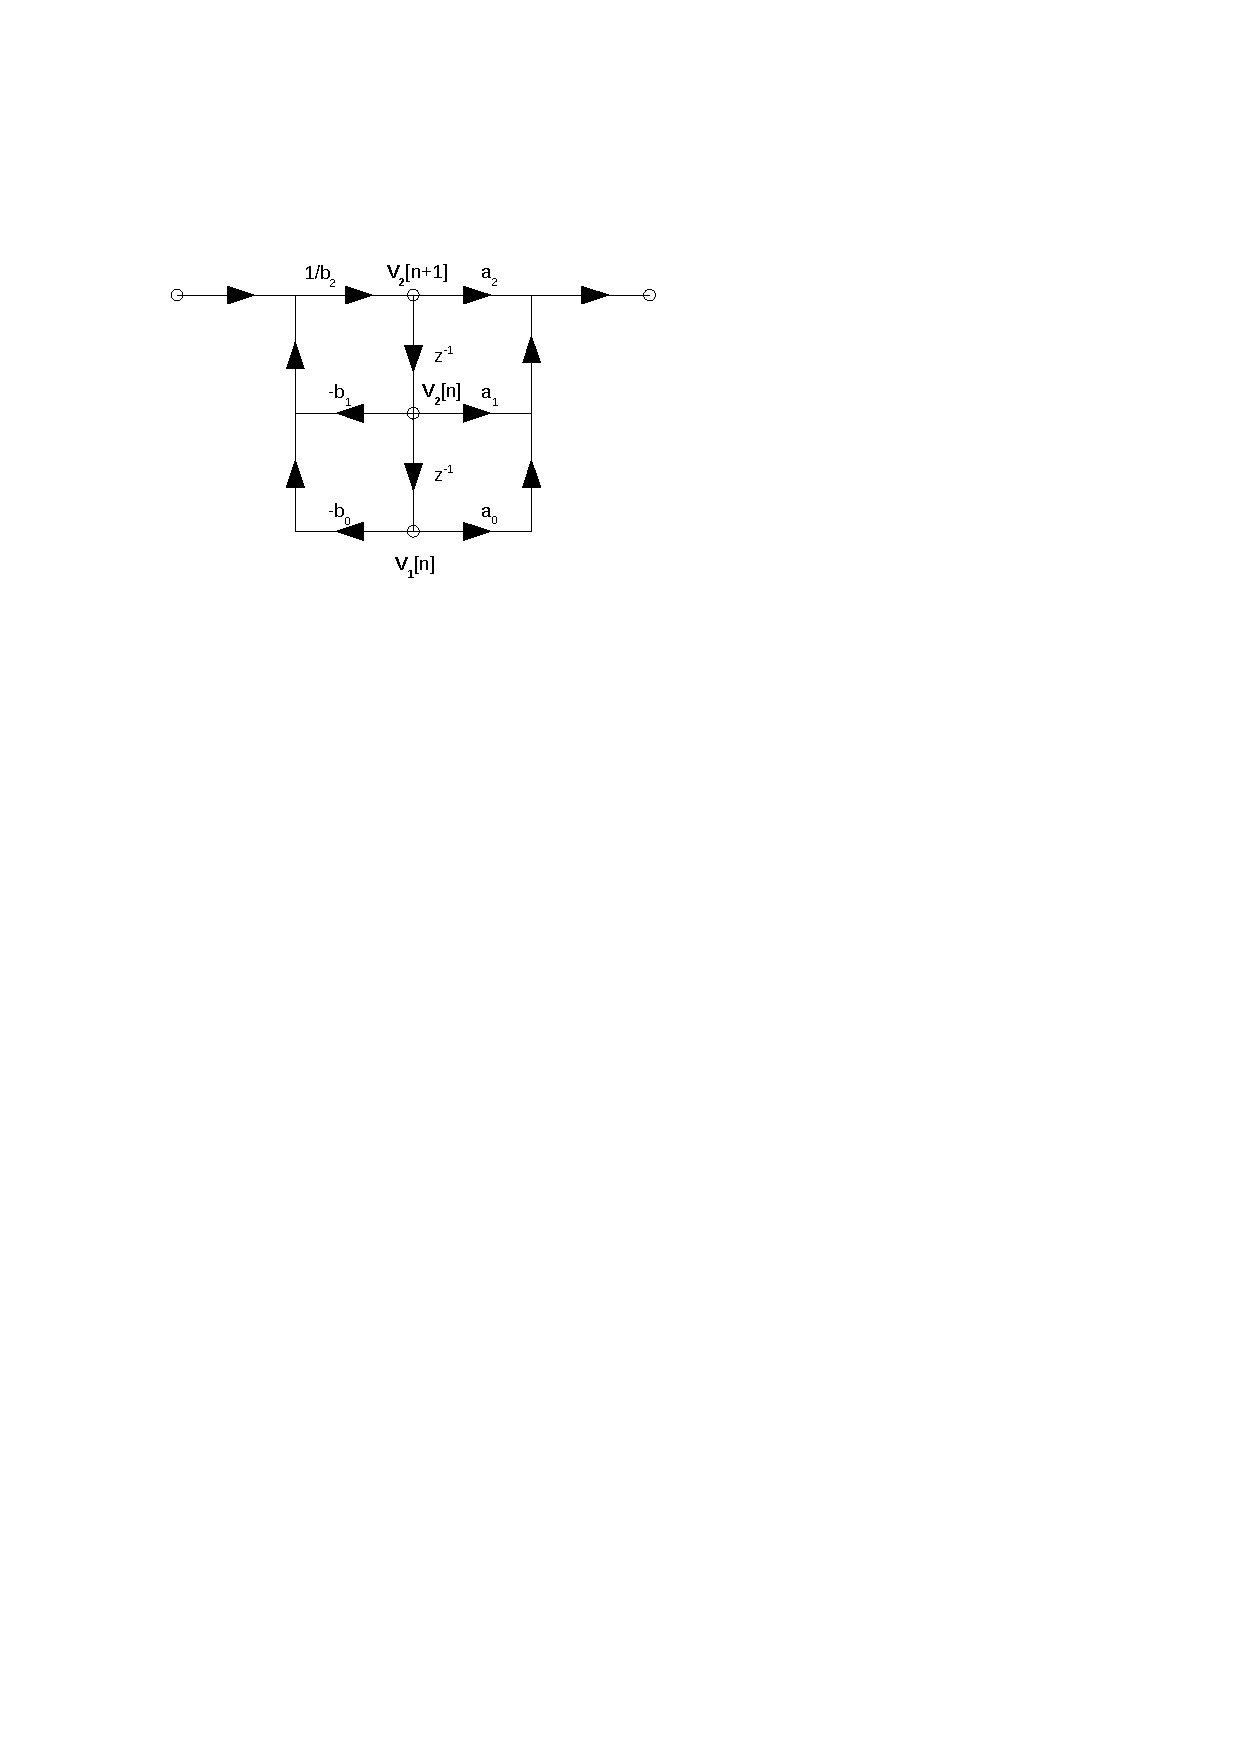
\includegraphics[scale=0.5]{data/2kanonicka}
  \end{center}
  \caption{Zlepšené Wilsonovo proudové zrcadlo.}
\end{figure}

Pro sazbu vektorových obrázků přímo v~\LaTeX{}u je možné doporučit balíček \href{https://www.ctan.org/pkg/pgf}{\texttt{TikZ}}.
Příklady sazby je možné najít na \href{http://www.texample.net/tikz/examples/}{\TeX{}ample}.
Pro vyzkoušení je možné použít programy QTikz nebo TikzEdt.




\chapter{Příklad sazby zdrojových kódů}

\section{Balíček \texttt{listings}}

Pro vysázení zdrojových souborů je možné použít balíček \href{https://www.ctan.org/pkg/listings}{\texttt{listings}}.
Balíček zavádí nové prostředí \texttt{lstlisting} pro sazbu zdrojových kódů, jako například:
%
\begin{lstlisting}[language={[LaTeX]TeX}]
\section{Balíček lstlistings}
Pro vysázení zdrojových souborů je možné použít
	balíček \href{https://www.ctan.org/pkg/listings}%
	{\texttt{listings}}.
Balíček zavádí nové prostředí \texttt{lstlisting} pro
	sazbu zdrojových kódů.
\end{lstlisting}
%
Podporuje množství programovacích jazyků.
Kód k~vysázení může být načítán přímo ze zdrojových souborů.
Umožňuje vkládat čísla řádků nebo vypisovat jen vybrané úseky kódu.
Např.:

\noindent
Zkratky jsou sázeny v~prostředí \texttt{seznamzkratek}:
\lstinputlisting[language={[LaTeX]TeX},nolol,numbers=left,firstline=1,lastline=1]{text/zkratky.tex}
%
Šířka textu druhého parametru udává šířku prvního sloupce se zkratkami.
Proto by měla být zadávána nejdelší zkratka nebo symbol.
Příklad definice zkratky \zk{symfvz} je na výpisu \ref{lst:symfvz}.

\iflanguage{czech}{\shorthandoff{-}}{}
\iflanguage{slovak}{\shorthandoff{-}}{}
\lstinputlisting[language={[LaTeX]TeX},frame=single,caption={Ukázka sazby zkratek},label=lst:symfvz,numbers=left,linerange={bsymfvz-\%\%\%\ esymfvz},includerangemarker=false]{text/zkratky.tex}
\iflanguage{slovak}{\shorthandon{-}}{}
\iflanguage{czech}{\shorthandon{-}}{}

\noindent
Ukončení seznamu je provedeno ukončením prostředí:
\lstinputlisting[language={[LaTeX]TeX},nolol,numbers=left,firstnumber=18,linerange=18]{text/zkratky.tex}

\vspace{\fill}

\noindent
{\bf Poznámka k~výpisům s~použitím volby jazyka \verb|czech| nebo \verb|slovak|:}\newline
Pokud Váš zdrojový kód obsahuje znak spojovníku \verb|-|, pak překlad může skončit chybou.
Ta je způsobená tím, že znak \verb|-| je v~českém nebo slovenském nastavení balíčku \verb|babel| tzv.\ aktivním znakem.
Přepněte znak \verb|-| na neaktivní příkazem \verb|\shorthandoff{-}| těsně před výpisem a hned za ním jej vraťte na aktivní příkazem \verb|\shorthandon{-}|.
Podobně jako to je ukázáno ve zdrojovém kódu šablony.


\clearpage

%\section{Výpis kódu prostředí Matlab}
Na výpisu \ref{lst:priklad.vypis.kodu.Matlab} naleznete příklad kódu pro Matlab, na výpisu \ref{lst:priklad.vypis.kodu.C} zase pro jazyk~C.

\lstnewenvironment{matlab}[1][]{%
\iflanguage{czech}{\shorthandoff{-}}{}%
\iflanguage{slovak}{\shorthandoff{-}}{}%
\lstset{language=Matlab,numbers=left,#1}%
}{%
\iflanguage{slovak}{\shorthandon{-}}{}%
\iflanguage{czech}{\shorthandon{-}}{}%
}

\begin{matlab}[frame=single,float=htbp,caption={Příklad Schur-Cohnova testu stability v~prostředí Matlab.},label=lst:priklad.vypis.kodu.Matlab,numberstyle=\scriptsize, numbersep=7pt]
%% Priklad testovani stability filtru

% koeficienty polynomu ve jmenovateli
a = [ 5, 11.2, 5.44, -0.384, -2.3552, -1.2288];
disp( 'Polynom:'); disp(poly2str( a, 'z'))

disp('Kontrola pomoci korenu polynomu:');
zx = roots( a);
if( all( abs( zx) < 1))
    disp('System je stabilni')
else
    disp('System je nestabilni nebo na mezi stability');
end

disp(' '); disp('Kontrola pomoci Schur-Cohn:');
ma = zeros( length(a)-1,length(a));
ma(1,:) = a/a(1);
for( k = 1:length(a)-2)
    aa = ma(k,1:end-k+1);
    bb = fliplr( aa);
    ma(k+1,1:end-k+1) = (aa-aa(end)*bb)/(1-aa(end)^2);
end

if( all( abs( diag( ma.'))))
    disp('System je stabilni')
else
    disp('System je nestabilni nebo na mezi stability');
end
\end{matlab}

\noindent
\begin{minipage}{\linewidth}


%\section{Výpis kódu jazyka C}

\begin{lstlisting}[frame=single,numbers=right,caption={Příklad implementace první kanonické formy v~jazyce C.},label=lst:priklad.vypis.kodu.C,basicstyle=\ttfamily\small, keywordstyle=\color{black}\bfseries\underbar,]
// první kanonická forma
short fxdf2t( short coef[][5], short sample)
{
	static int v1[SECTIONS] = {0,0},v2[SECTIONS] = {0,0};
	int x, y, accu;
	short k;

	x = sample;
	for( k = 0; k < SECTIONS; k++){
		accu = v1[k] >> 1;
		y = _sadd( accu, _smpy( coef[k][0], x));
		y = _sshl(y, 1) >> 16;

		accu = v2[k] >> 1;
		accu = _sadd( accu, _smpy( coef[k][1], x));
		accu = _sadd( accu, _smpy( coef[k][2], y));
		v1[k] = _sshl( accu, 1);

		accu = _smpy( coef[k][3], x);
		accu = _sadd( accu, _smpy( coef[k][4], y));
		v2[k] = _sshl( accu, 1);

		x = y;
	}
	return( y);
}
\end{lstlisting}
\end{minipage}







\chapter{Obsah přiloženého CD}
Nezapomeňte uvést, co čtenář najde na přiloženém médiu.
Je vhodné okomentovat obsah každého adresáře, specifikovat, který soubor obsahuje důležitá nastavení, který soubor je určen ke spuštění atd.
Také je dobře napsat, v~jaké verzi software byl kód testován (např.\ Matlab 2010b).

Pokud je souborů hodně a jsou organizovány ve více složkách,  je možné pro výpis adresářové struktury použít balíček \href{https://www.ctan.org/pkg/dirtree}{\texttt{dirtree}}.

\dirtree{%.
.1 /\DTcomment{kořenový adresář přiloženého CD}.
.2 loga\DTcomment{loga školy a fakulty}.
.3 FEKT-spec-color.eps.
.3 FEKT-spec-color.pdf.
.3 logolink-op\_vavpi.png.
.3 RE-spec-color.eps.
.3 RE-spec-color.pdf.
.3 SIX\_logo\_zahlavi.png.
.2 obrazky\DTcomment{ostatní obrázky}.
.3 soucastky.eps.
.3 soucastky.png.
.3 spoje.eps.
.3 spoje.png.
.3 ZlepseneWilsonovoZrcadloNPN.eps.
.3 ZlepseneWilsonovoZrcadloNPN.png.
.3 ZlepseneWilsonovoZrcadloPNP.eps.
.3 ZlepseneWilsonovoZrcadloPNP.png.
.2 pdf\DTcomment{pdf stránky generované informačním systémem}.
.3 student-desky.pdf.
.3 student-titulka.pdf.
.3 student-zadani.pdf.
.2 text\DTcomment{zdrojové textové soubory}.
.3 literatura.tex.
.3 prilohy.tex.
.3 reseni.tex.
.3 uvod.tex.
.3 vysledky.tex.
.3 zaver.tex.
.3 zkratky.tex.
.2 navod-sablona\_FEKT.pdf\DTcomment{návod na používání šablony}.
.2 obhajoba.tex\DTcomment{hlavní soubor pro sazbu prezentace k~obhajobě}.
.2 readme.txt\DTcomment{soubor s~popisem obsahu CD}.
.2 sablona.tex\DTcomment{hlavní soubor pro sazbu kvalifikační práce}.
.2 thesis.sty\DTcomment{balíček pro sazbu kvalifikačních prací}.
}

\chapter{Uživatelský manuál programu Sound Analyzer}


\section{Slovníček pojmů užitých v této kapitole}

\subsection{Frequency indexes}

Indexy kmitočtů které budou počítány. Jsou to čísla $n$ ze vzorce \ref{vztah:DFT}.


\subsection{Sampling frequency}

Vzorkovací kmitočet.

\subsection{Scale}

Měřítko specifikuje zobrazený rozsah grafů a je znázorněno na pravítkách.

\subsection{Segment length}
\label{sec:segmentlegth}

Segmentem je myšlen vektor určité délky, reprezentující část signálu. Komponenta \emph{Recorder} čte ze vstupu (nebo přehrává) právě po úsecích této délky.

\subsection{Segment overlap}
\label{sec:segmentoverlap}

Komponenta \emph{Goertzel} umí pracovat s větší délkou segmentu než s tou, kterou načte ze vstupu. \emph{Segment overlap} je délka z předchozích vzorků, o kterou se rozšíří segment (vstupní vektor).


\section{Okno aplikace}

Na obrázku \ref{obr:manual1} vidíme základní obrazovku programu \emph{Sound Analyzer}.
Pravítka slouží k odečítání časů a velikostí amplitud jednoho nebo dvou grafů. Spodní lišta slouží k přepínání pohledů na signál. Konečně navigační pole slouží ke konfiguraci a zobrazuje důležité statistické informace o signálu. 

\begin{figure}
  \begin{center}
    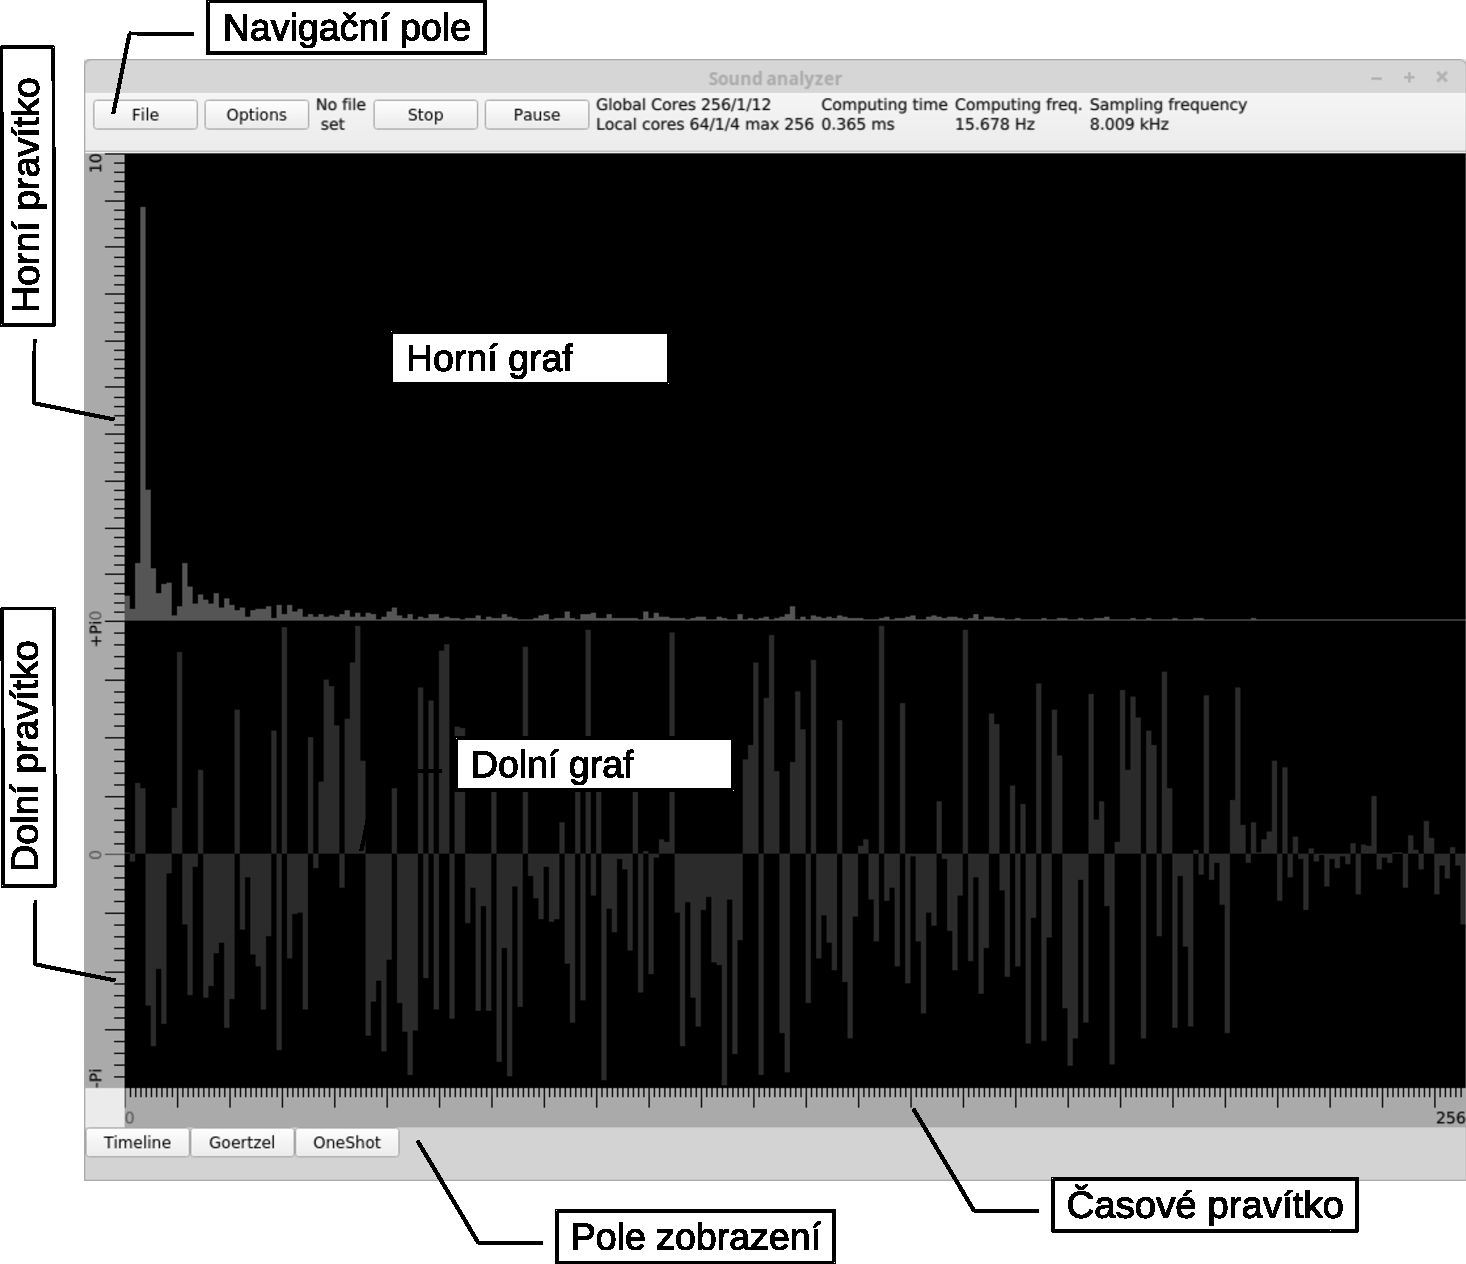
\includegraphics[scale=.65]{obr/manual1}
  \end{center}
  \caption{Pohled na aplikaci Sound Analyzer}
  \label{obr:manual1}
\end{figure}

\section{Horní graf}
\label{sec:topgraph}

Horní graf má dva režimy zobrazení. V zobrazení typu \emph{Goertzel} a \emph{OneShot} reprezentuje amplitudu. V režimu zobrazení \emph{Timeline} zobrazuje průběh signálu levého kanálu.
Ten se neposouvá, jinak řečeno, vždy když se načte segment, je zobrazen místo segmentu předcházejícího. Pokud je rychlost změn větší než obnovovací rychlost GUI knihovny \emph{Qt} zobrazený segment je zahozen a zobrazuje se ten poslední.

Zobrazení \emph{Timeline} může být dvougrafové(stereo) nebo grafem přes celou velikost okna(Mono). To je možno nastavit přepínačem \emph{Channels} a kartě \emph{Recorder} z dialogu \emph{Options}.


Měřítko v horizontálním směru je popsané v sekci časové pravítko \ref{sec:timeruler}.


Měřítko ve vertikálním směru je popsané v sekci Dolní a horní pravítko \ref{sec:vertruler}.


\section{Dolní graf}


I dolní graf má dva režimy zobrazení. V zobrazení typu \emph{Goertzel} a \emph{OneShot} reprezentuje fázi. V režimu zobrazení \emph{Timeline} zobrazuje průběh signálu pravého kanálu. Ten se cyklicky překresluje, jak je blíže popsáno o horního grafu \ref{sec:topgraph}.

Měřítka, stejně jako u grafu horního jsou popsány v sekcích o pravítkách  \ref{sec:timeruler}, \ref{sec:vertruler}.

\section{Horní a dolní pravítko}
\label{sec:vertruler}

V zobrazení typu \emph{Goertzel} a \emph{OneShot} reprezentuje amplitudu v rozsahu od $0$ do $y_{max}$. V režimu zobrazení \emph{Timeline} zobrazuje průběh signálu v rozsahu $-y_{max}$,$y_{max}$. Rozsah $y_{max}$ lze měnit jednak klávesovými zkratkami, jednak rozbalovacím seznamem \emph{Scale} na kartě \emph{General} z dialogu \emph{Options}.

\section{Časové pravítko}
\label{sec:timeruler}

V režimu \emph{Timeline} je na vodorovné ose vynesen počet vzorků které jsou najednou načteny ze vstupu. Je to současně nastavená hodnota \emph{Segment length} na kartě \emph{Recorder} v dialogu \emph{Options}. V režimu \emph{Goertzel} je na této ose počet počítaných harmonických, uvedených v seznamu \emph{Frequency indexes} na kartě \emph{Goertzel} v dialogu \emph{Options}. V režimu \emph{OneShot} se počítají všechny možné kmitočty signálu popsaném v souboru z \emph{Matlabu}. Na vodorovné ose je tedy počet kmitočtů, číselně roven délce zkoumaného signálu.

\section{Pole zobrazení}

V \emph{poli zobrazení} jsou tři tlačítka reprezentující tři režimy. Jsou to jediné akce, které můžete provádět za běhu.


Kromě změny zobrazení, tyto tlačítka přestavují toky dat mezi komponentami, jak je patrno z obrázku \ref{sec:sablockscheme}. Proto se při přepnutí z jednoho režimu do druhého a~zpět zobrazí implicitní sinus. Při přepnutí fronty se totiž segment se zobrazovanými daty musí vrátit.

\subsection{Timeline}

Režim \emph{Timeline} zobrazuje syrová data ze vstupu tak jak jdou za sebou. Jeden graf zobrazuje jeden segment. Zobrazení se s přibývajícím čase neposouvá, ale jen se překreslí aktuální segment.

Pokud je frekvence příchozích segmentů vyšší než je zobrazovací frekvence knihovny \emph{Qt}, tak se segmenty jednoduše zahodí (a vidět je ten poslední).

\subsection{Goertzel}

Režim \emph{Goertzel} zobrazuje spektrum signálu, respektive jen jeho požadované harmonické. Na horizontální ose najdeme počet počítaných harmonických.

\subsection{OneShot}

Režim \emph{OneShot} je kompletní spektrum signálu dodaného ze souboru \emph{matlabu}.
Pokud je v tomto souboru více vektorů se signály, zobrazen se jen ten poslední.

\section{Navigační pole}

Zde uvedu informační a ovládací prvky navigačního pole zleva doprava.

\subsection{Tlačítko File}

\subsubsection{Open for reading}

Klasickým \emph{File dialogem} si můžeme vybrat \emph{wav} soubor, který bude přehráván po stisknutí tlačítka \emph{Start}. Protože přehráváním se současně udává takt, bude program i nadále fungovat v reálném čase. Je možné mít otevřený soubor buď jen pro čtení nebo jen pro zápis, nikoli oba současně.

\subsubsection{Open for writing}

Klasickým \emph{File dialogem} si můžeme vybrat \emph{wav} soubor, do kterého budou ukládány načtené vzorky ze vstupu. V případě že výstupní zařízení není schopno ukládat požadované množství dat, bude výstupní soubor poškozený. 

\subsubsection{Close file}

Tímto zrušíte obě předchozí volby. Nyní se bude počítat spektrum jen ze vstupu.

\subsubsection{Process mat file}

Tato funkce je v programu \emph{Sound Analyzer} nejen pro ladící účely. Provede spočtení všech harmonických signálu dodaného v souboru typu \emph{mat} vytvořeném v prostředí \emph{matlab}.

Soubor typu \emph{mat} může obsahovat více vektorů. V takovém případě se provede výpočet spektra všech vektorů, ale vidět v pohledu \emph{OneShot} je pouze poslední.

Výstupní soubor je pojmenovaný jako $<vstupní soubor>\_ap$. V tomto souboru jsou dvě,
respektive dvakrát více vektorů než v souboru vstupním (amplituda a fáze). Jméno vektoru s amplitudami
 je $<vstupní vektor>\_am$ a vektory s fázemi mají jména $<vstupní vektor>\_ph$.

\subsubsection{Quit}

Konec programu.

\subsection{Tlačítko Options}

Spustí dialog nastavení. Více v sekci \emph{Dialog nastavení} \ref{sec:settingdialog}

\subsection{Jméno souboru pro zápis/čtení}

Zde je jméno souboru pro zápis/čtení a informace o tom, v jakém režimu souborové operace jsou (zápis/čtení/nic).

\subsection{Tlačítko Start}

Tlačítko \emph{Start} slouží ke startu jak skenování vstupu, tak počítání spektra.
Aby se počítalo spektrum, je nutné zobrazit režim \emph{Goertzel}, jinak načtená data nejdou přes Goertzelův algoritmus, ale pouze se zobrazují.

Teprve začátkem zaznamenávání nebo přehrávání se aplikují změny v dialogu nastavení.

Kliknutím se text na tlačítku změní na \emph{Stop}.

\subsection{Tlačítko Pause}

Tlačítko \emph{Pause-Continue} funguje i když zrovna není zapnuto skenování. To znamená že když je stav \emph{zapauzovaný} a následně kliknete na tlačítko \emph{Start}, skenování se zinicializuje, ale vlastní skenování nepoběží.

\subsection{Počet jader použitých při výpočtech}
\label{sec:nkernels}

V tomto okénku je sedm údajů: Globální $N/C/M$, lokální $N/C/M$ a maximální počet jader současně spustitelných.  $N$ je počet počítaných kmitočtů, $C$ je počet kanálů a konečně $M$ je počet mezisoučtů. Globální počet jader je tedy celkový požadavek na výpočet a jeho velikost je $N\times C\times M$. Tři souřadnice udávají počet jader se v terminologii  \emph{OpenCL} nazývají $NDrange$. Naproti tomu lokální $NDRange$ je skutečná počet jader použitých současně pro výpočet. Určitě tedy platí, že $globální NDRange \geq lokální NDRange$. Je tu ještě jedno omezení. Globální souřadnice $NDRange$ 
musí být celočíselný násobek lokální souřadnice $NDRange$.

\subsection{Průměrný čas výpočtu spektra}

Vlákno programu \emph{Sound Analyzer}, které v cyklu počítá některé harmonické složky, obsahuje jednoduchou počítací smyčku. Jedna její iterace trvá právě tento zobrazený čas.

\subsection{Průměrná frekvence výpočtu spektra}

Jedná se o frekvenci, se kterou se provádí výpočty. Měla by být někde okolo\\
 $f_{vz} / <délka segmentu>$.

\subsection{Průměrná vzorkovací frekvence}
\label{sec:avgsamplingfreq}

Je spočtená hodnota braná z komponenty \emph{recorder}. Měla by být podobná
nastavenému \emph{vzorkovacímu kmitočtu}.

\section{Klávesové zkratky}

\begin{tabular}{|c|l|}
\hline
+&Zvýšení rozsahu vertiálního měřítka\\
-&Snížení rozsahu vertikálního měřítka\\
S&Start, Stop\\
space&Pause, Continue\\
\hline 
\end{tabular}


\section{Dialog nastavení}
\label{sec:settingdialog}


\subsection{Karta General}

\subsubsection{Automatic hide}

Automatické schovávání je jen hříčka pro \uv{hezčí} zobrazení, bez okraje okna, \emph{navigačního pole} a \emph{pole zobrazení}.

\subsubsection{Scale}

\emph{Vertikální měřítko} grafu se aplikuje okamžitě. Je to jedna z mála výjimek v dialogu \emph{Nastavení}. Pro rychlejší manipulaci s měřítkem jsou v programu klávesové zkratky $+,-$.

\subsection{Karta Recorder}

\emph{Recorder} je komponenta zodpovědná za načítání vzorků ze zvukového zařízení, případně přehrávání zvukového souboru. V případě že je to povoleno, posílá ještě data k uložení do souboru.

\subsubsection{Bits per sample}

Knihovna \emph{OpenAL} nabízí jen dvě možnosti přesnosti každého vzorku, 8bitovou a~16bitovou. Oba jsou to celočíselné typy.

\subsubsection{Channels}

Program \emph{Sound Analyzer} podporuje jak mono, tak stereo záznam, tak i přehrávání i~výpočet spektrálních čar. Modrou barvou je značen levý kanál, červenou pak pravý.

\subsubsection{Device}

Zde jde nastavit jen zařízení \emph{OpenAL Soft}. Knihovna \emph{OpenAL} nikdy žádné jiné zařízení nenabídla.

\subsubsection{Capture device}

\emph{Zařízení pro záznam zvuku} jsou obvykle tři. Výchozí je vždy \uv{vnitřní zvukový systém}, což je vždy mikrofon. Další zařízení, které tam vždy najdeme, je \uv{monitor vnitřního zvukového systému}, což je standardní zvukový výstup. Když ale zkusíme tento vstup nahrávat, zjistíme, že je nějak poškozen. Protože výchozí vstupní zařízení zvuk nedeformuje, jsem názoru, že jde o ochranu proti kopírování. Tento vstup totiž není zatížen ani minimálním šumem. Jako poslední je obvykle vstup, \uv{monitor HDMI výstupu}. Ten je nějak zkreslen podobně jako vstup předchozí.

\subsubsection{Sampling frequency}

Tato vzorkovací frekvence je použita pro inicializaci \emph{recorderu}. Pokud se podíváme na kmitočet spočtený \ref{sec:avgsamplingfreq}, zjistíme že pro \emph{zařízení-monitory}, nejsou tyto kmitočty totožné. V tom je to zkreslení.

\subsubsection{Segment length}

Délka segmentu (vektor vstupního signálu) v počtu vzorků. Více o něm je v sekci \emph{segment length} ve slovníčku pojmů \ref{sec:segmentlegth}.

\subsection{Karta Goertzel}

Tato karta se týká výhradně výpočtu spektrálních čar a knihovny \emph{OpenCL}.

\subsubsection{Segment overlap}

Počet vzorků, o které se rozšíří načtený segment. Více je ve slovníčku \emph{segment overlap} \ref{sec:segmentoverlap}.

\subsubsection{Frequency indexes}

V tomto textovém poli je seznam indexů spektrálních čar počítaného spektra. Nic nebrání tomu počítat jen stejnosměrnou složku (index 0) nebo několik málo kmitočtů, které nejdou po sobě. Jednotlivé celočíselné indexy jsou odděleny \uv{;} a pro lepší přehlednost mohou obsahovat libovolný počet přechodů na nové řádky.

\subsubsection{Tlačítko Set All}

Snazšího vyplnění předcházejícího pole dosáhneme tlačítkem \emph{Set All}. To nahradí jakýkoli obsah pole \emph{frequency indexes} indexy $0$ až $(segment\_length + segment\_overlap)$.

\subsubsection{Přepínač Device}

Tímto říkáme knihovne \emph{OpenCL}, zda požadujeme provádět výpočty hlavním procesorem nebo grafickým čipem.

\section{Příklad použití}

Předpokládejme, že bude chtít počítat stejnosměrnou složky signálu a současně amplitudu na kmitočtu 1kHz. Vzorkovací kmitočet použiji 8kHz.

Délku segmentu si zvolím. Například délka 200 vzorků by se načítala 200/8000s = 25ms. To je tak maximální doba, při které může třeba řečový signál považovat za stacionární.

Nejnižší, základní kmitočet, který jsem takto schopen měřit je 8000/200 = 40Hz. Nás ale zajímají indexy 0 - stejnosměrná složka a 1000Hz = 25 $\times$ 40Hz. Druhý index je tedy 25.

Ve shodě s předchozím nastavíme v dialogu \emph{nastavení} toto:\\

\begin{tabular}{|l|l|}
\hline
Bits per sample&16bit\\
Channels&Mono\\
Device&OpenAl Soft\\
Capture device&Vnitřní zvukový systém analogové stereo\\
Sampling frequency&8000\\
Segment length&200\\
Segment overlap&0\\
Frequency indexes&0;25;\\
Device&GPU\\
\hline 
\end{tabular}




\chapter{Instalace projektu - spuštění aplikace}
\label{kap:instalaceprogramu}

K aplikaci není přiložen žádný instalační program. Není potřeba. Spouští se jen spustitelným souborem \emph{SoundAnalyzer} v adresáři téhož jména. Zabalený archiv s~programem naleznete na přiloženém CD disku. Stačí jej jen rozbalit.


Nicméně pro správnou funkci je třeba mít správně nainstalované knihovny \emph{OpenCL} a \emph{OpenGL}. Knihovny \emph{OpenGL} a \emph{OpenCL} dodává výrobce grafické karty, tudíž je problematické napsat nějaký návod na její nainstalování, nebo dokonce nějaký instalační skript. Obecně lze říci, že v linuxu je lepší používat proprietární ovladače od výrobců grafických čipů něž ovladače volně šiřitelné. Jejich instalace ale může přinést potíže, mně třeba pokus o instalaci ovladače od NVidie způsobil nefunkčnost operačního systému a musel jsem tento znovu nainstalovat.

\section{GPU AMD}

Na \url{http://support.amd.com/en-us/download/linux} lze stáhnout ovladač \emph{fglrx}. S jeho instalací jsem neměl žádné problémy. Možná bude potřeba nainstalovat i~\emph{OpenCL} z adresy \href{http://developer.amd.com/tools-and-sdks/opencl-zone/amd-accelerated-parallel-processing-app-sdk/}{developer.amd.com} a je rovněž na přiloženém CD nosiči. Instalace je bez problémů.

\section{GPU NVidia}

Ovladač Nvidia je nyní ve standardním repozitáři Ubuntu a Mint a to v poslední verzi \emph{375}. Když instalujete nové Ubuntu nebo Mint, je třeba před instalací spustit správce ovladačů a vybrat \uv{používat NVidia 340}. Když Linux nainstalujete a připojíte k síti a opět spustíte výše jmenovaný program, nabídne vám již aktuální verzi \emph{375}. OpenCl je součátí CUDA a je také ve standardním repozítáři.
Nainstalujete zadáním:

\begin{Verbatim} 
sudo apt-get install libcuda1-375
\end{Verbatim}

\chapter{Instalace projektu - pokračování ve vývoji}
\label{kap:instalace}

\section{Instalace GNU C++}

Přestože knihovny \emph{OpenCV} a \emph{OpenCL} jsou multiplatformní, rozhodl jsem se pro operační systém Linux, distribuce Mint 17. Vyhnul jsem se konstrukcím platformně závislým, takže je možná přenositelnost na jiné operační systémy. Jako překladač jsem zvolil \emph{GCC}, a to ze stejného důvodu jako předchozí, je platformně nezávislý a~je v každé distribuci Linuxu jako jeden ze základních balíčků. Mně stačilo
k instalaci napsat:

\begin{verbatim}
sudo apt-get install build-essential
\end{verbatim}

a potom...

\begin{Verbatim}
sudo apt-get install g++
\end{Verbatim}


Pro Windows existuje disrtibuce GNU cygwin, kterou je možno stáhnout a nainstalovat z webu \url{sourceware.org/cygwin}.


Důležité je nezapomenout zaškrtnout \emph{devel} a \emph{debug} v seznamu balíčků k instalaci.



\section{Verzovací systém Git}

Verzovací systém Git používám nejen v zaměstnání, ale i v domácích
projektech a~má své místo i v této práci. Může být důležité moci se v případě
nutnosti vrátit k~předchozím verzím projektu.

Git je standardní balíček snad všech distribucí. Instaluje je jako obvykle napsáním

\begin{Verbatim} 
sudo apt-get install git
\end{Verbatim}

S klíči se zachází standardním způsobem, měly by být uloženy v
adresáři \functionname{\textasciitilde/.ssh}.

Vytvořil jsem speciální repozitář na svém testovacím serveru.
Přihlašovat se jde výhradně pomocí klíče, který najdete na CD--příloze této práce. Projekt stačí už jen naklonovat příkazem,

\begin{Verbatim} 
git clone virtualbox@46.167.245.175:dp
\end{Verbatim}

přesněji, pomocí klíče na CD

\begin{Verbatim} 
ssh-agent sh -c 'ssh-add <cesta>/virtualbox_rsa;
git clone virtualbox@46.167.245.175:dp'
\end{Verbatim}


\section{Qt Creator}


Qt Creator je nedílnou součástí vývojového kitu knihovny Qt. Nyní je již verze
5.8, já jsem ale použil verzi 5.5.1, která je podporována ve standardních repozitářích linuxu, konkrétně jsem vyzkoušel Mint 18.1 a Ubuntu 16.04.

Instalační baliček je součástí přiloženého CD a je možné ho rovněž stáhnout ze stránek \url{qt.io}.


Celá aplikace je napsaná v prostředí \emph{Qt Creator}. \emph{Qt creator} má problémy s~vizuálním návrhářem, a to takové, že je zcela nepoužitelný a layout dialogů je nutné psát textově v jazyce /emph{qml}. Stále je však možno použít prostředí \emph{QtCreatoru} pro psaní textu a překlad programu.


\section{OpenGL}


Instalaci proprietárního ovladače a knihovny \emph{OpenGL} jsem popsal v kapitole \emph{instalace programu} \ref{kap:instalaceprogramu}.

Tím ale máme v systému knihovny, nikoli už ale  hlavičkové soubory pro jejich použití. Já jsem napsal pro začátek vývoje v OpenGL toto:

\begin{Verbatim} 
sudo apt-get install freeglut3
sudo apt-get install freeglut3-dev
sudo apt-get install binutils-gold
sudo apt-get install mesa-common-dev
sudo apt-get install libglew1.5-dev libglm-dev
\end{Verbatim}

\section{OpenAL}

Instalace vývojových balíčků pro knihovnu OpenAl je velmi jednoduchá, prakticky nikdy se nestalo že by něco nefungovalo. V Ubuntu jsou to standardní balíčky:

\begin{Verbatim} 
sudo apt-get install libopenal-dev
sudo apt-get install libalut-dev
\end{Verbatim}

\section{OpenCL}

Tak jako \emph{OpenGL} i \emph{OpenCL} je poskytována výrobcem grafického čipu. Je tedy nutné 
mít dobře nainstalovanou grafickou kartu s proprietárními ovladači.

Ve standardních repozitářích Ubuntu je následující balíček...

\begin{Verbatim} 
sudo apt-get install ocl-icd-libopencl1,
\end{Verbatim}

ten nainstaluje nějakou \emph{OpenC}L knihovnu. Program potom jde spustit, ale inicializace vrátí chybu, není platforma, takže není možno provádět výpočet ani softwarově.


SDK pro \emph{OpenCL} na grafických čipech \emph{AMD} je možno stáhnout z adresy \href{http://developer.amd.com/tools-and-sdks/opencl-zone/amd-accelerated-parallel-processing-app-sdk/}{developer.amd.com} a je rovněž na přiloženém CD nosiči. Instalace je bez problémů.
Jediné co potom musíte udělat, je nastavení cesty ke hlavičkovému souboru a knihovně v případě, že chcete použít její vývojovou verzi. U mně to bylo například:\\
\emph{/opt/AMDAPPSDK-2.9-1/include}.


SDK pro \emph{OpenCL} na grafických čipech \emph{NVidia} je v Ubuntu ve standardních repozitářích a
je spojena s implementací knihovny \emph{CUDA}. Pro instalaci stačí napsat:

\begin{Verbatim} 
sudo apt-get install libcuda1-375
sudo apt-get install nvidia-cuda-dev
\end{Verbatim}
kde 375 je jméno verze ovladače grafického čipu NVidia.

\chapter{Slovníček pojmů knihovny OpenCL}

Tato kapitola je výtahem z dokumentace k openCL (\cite{opencl}).
Úplnou dokumentaci lze najít \url{kronos.org}.

\section{Application -- Aplikace}
\label{sec:application}

Kombinace programů běžících, jak na \emph{hostitelském zařízení (host device)} (viz termín \ref{sec:host}), tak na openCL \emph{zařízení (device)}  (viz termín \ref{sec:device}).

\section{Blocking a Non-Blocking Enqueue API calls -- Blokující a~neblokující příkazy }
\label{sec:blockunblocapicall}

\emph{Neblokující} \emph{příkaz (command)} (viz termín \ref{sec:command}) ve frontě volání vloží \emph{příkaz} (viz termín \ref{sec:command}) do
\emph{příkazové fronty} (viz termín \ref{sec:commandqueue}) a~okamžitě vrátí řízení \emph{hostiteli} (viz termín \ref{sec:host}). \emph{Blokující}
příkaz ve frontě nevrátí řízení hostiteli, dokud není \emph{příkaz} (viz termín \ref{sec:command}) proveden.

\section{Barrier  -- Bariéra}
\label{sec:barrier}

Jsou dva druhy \emph{bariér (barriers)} (viz termín \ref{sec:barrier}) -- bariéra \emph{fronty zpráv} (viz termín \ref{sec:commandqueue}) a~
bariéra \emph{pracovní skupiny (work-group)} (viz termín \ref{sec:workgroup}). 
\begin{itemize}
\item \emph{OpenCL API} poskytuje
funkci zařazení \emph{bariéra fronty zpráv} (viz termín \ref{sec:commandqueuebarrier}). Tento příkaz zajistí, že
předchozí příkazy jsou provedeny před tím, než začne příkaz následující.
\item \emph{OpenCL C} programovací jazyk poskytuje vestavěnou funkci \emph{bariéra pracovní skupiny} (viz termín \ref{sec:workgroupbarrier}). Tato bariéra může býti volána \emph{jádrem (kernel)} (viz termín \ref{sec:kernel}) pro zajištění
synchronizace mezi \emph{pracovními členy (work-items)} (viz termín \ref{sec:workitem}) v~\emph{pracovních skupinách} (viz termín \ref{sec:workgroup}) provádějících \emph{jádra} (viz termín \ref{sec:kernel}). Všechny \emph{pracovní členy} v~\emph{pracovní skupině}
musí provést tuto synchronizaci, než bude možno pokračovat v~provádění následujících příkazů.
\end{itemize}



\section{Buffer object  -- Buffer}
\label{sec:buffer}
Buffer je paměťový objekt, ve kterém je uložena souvislá řada bytů. Tento buffer
je přístupný použitím ukazatele z \emph{jádra} prováděném na~\emph{zařízení}. S~těmito buffery
může býti manipulováno použitím OpenCL API funkcí. Buffer zapouzdřuje následující
informace:

\begin{itemize}
\item Velikost v~bytech.
\item Parametry popisující uložení v~paměti a~ve které oblasti je alokován.
\item Buffer data.
\end{itemize}

\section{Built-in kernel -- Vestavěné jádro}
\label{sec:builtinkernel}

\emph{Vestavěné jádro} je je \emph{jádro} (viz termín \ref{sec:kernel}) prováděné na~openCL \emph{zařízení} (viz termín \ref{sec:device}) nebo \emph{speciálním zařízení (custom device)} (viz termín \ref{sec:customdevice}) pevně daným hardwarem nebo firmwarem. Aplikace může používat \emph{vestavěná jádra} nabízená \emph{zařízeními} nebo \emph{speciálními zařízeními}. \emph{Objekty programů 
(program objects)} (viz termín \ref{sec:programobject}) mohou obsahovat jen \emph{jádra} napsané v~jazyce openCL C nebo \emph{vestavěná jádra}, ale nikdy ne obojí. Více viz \emph{jádra} (viz termín \ref{sec:kernel}) a~\emph{programy} (viz termín \ref{sec:program}).

\section{Command -- Příkaz}
\label{sec:command}
Operace v~openCL jsou posílány k provedení do \emph{fronty příkazů (command queue)} (viz termín \ref{sec:commandqueue}).
Například openCL \emph{příkazy} (viz termín \ref{sec:command}) pověřují \emph{jádra (kernels)} (viz termín \ref{sec:kernel}) k provedení
na~\emph{výpočetním zařízení} (viz termín \ref{sec:device}), manipulaci s~paměťovými objekty atd.

\section{Command Queue -- Fronta příkazů}
\label{sec:commandqueue}
\emph{Fronta příkazů (command queue)} (viz termín \ref{sec:commandqueue}) je objekt ve kterém jsou uloženy příkazy,
které budou vykonány na~určitém \emph{zařízení} (viz termín \ref{sec:device}). \emph{Fronta příkazů} (viz termín \ref{sec:commandqueue}) je vytvořena 
na~určitém \emph{zařízení} s~určitým \emph{kontextem (context)} (viz termín \ref{sec:context}). \emph{Příkazy} (viz termín \ref{sec:command}) jsou zařazeny
do \emph{fronty příkazů} (viz termín \ref{sec:commandqueue})  v~pořadí, ale vykonat se mohou v~tomto pořadí nebo
v pořadí jiném. Více viz \emph{provádění v~pořadí (in-order execution)} (viz termín \ref{sec:inorderexecution})  a
\emph{provádění mimo pořadí (out-order execution)} (viz termín \ref{sec:outoforderexecution}).


\section{Command Queue Barrier -- Bariéra fronty příkazů}
\label{sec:commandqueuebarrier}

Více na~\emph{bariéra (barrier)}  (viz termín \ref{sec:barrier}).


\section{Compute device memory -- Paměť výpočetního zařízení}
\label{sec:computedevicememory}

Jedno \emph{zařízení} (viz termín \ref{sec:device}) může mít připojeno jednu nebo více pamětí.

\section{Compute unit -- Výpočetního jednotka}
\label{sec:computeunit}

OpenCL \emph{zařízení} (viz termín \ref{sec:device}) může mít jednu nebo více \emph{výpočetních jednotek (compute units)} (viz termín \ref{sec:computeunit}). \emph{Pracovní skupina (work-group)} (viz termín \ref{sec:workgroup}) je provedena na~jedné výpočetní jednotce. Výpočetní jednotka je tvořena jedním nebo více \emph{procesorovým prvkem 
(processing element)} (viz termín \ref{sec:processingelement}) a~\emph{lokální pamětí (local memory)} (viz termín \ref{sec:localmemory}). Výpočetní jednotka
také může obsahovat filtr textur, který může být přístupný z  \emph{procesorových prvků} (viz termín \ref{sec:processingelement}).


\section{Concurrency -- Souběžnost}
\label{sec:concurrency}

Vlastnost systému, ve kterém je nějaká skupina úloh současně aktivní a~provádí nějakou akci. Pro využití \emph{souběžného provádění} (viz termín \ref{sec:concurrency}) programů, musí programátor
identifikovat možné problémy \emph{souběžného} zpracování, zahrnout je do svých zdrojových
kódů a~využít synchronizačních možností zařízení.

\section{Constant memory -- Paměť konstant}
\label{sec:constantmemory}
Oblast v~paměti přístupná \emph{jádru} (viz termín \ref{sec:kernel}), která je za~běhu \emph{jádra} konstantní. Tuto paměť alokuje i inicializuje 
\emph{hostitel} (viz termín \ref{sec:host}).

\section{Context -- Kontext}
\label{sec:context}

Prostředí, ve kterém se provádí \emph{jádra} (viz termín \ref{sec:kernel}) a~doména,
ke které se váží synchronizační a~\emph{paměťové objekty} (viz termín \ref{sec:memoryobjects}).
Kontext zahrnuje množinu \emph{zařízení}, příslušnou paměť
k těmto \emph{zařízením}, proměnné vázající se k těmto pamětem a~jednu nebo více \emph{front příkazů} (viz termín \ref{sec:commandqueue}).

\section{Custom device -- Speciální zařízení}
\label{sec:customdevice}

\emph{Speciální zařízení} má podporu openCL runtime, ale není možné pro něj psát programy v~openCL C.
Tyto zařízení jsou obvykle vysoce efektivní pro
určité typy úloh. Mohou mít vlastní překladač.
Pokud ho nemají, je možné spouštět pouze
\emph{vestavěná jádra} (viz termín \ref{sec:builtinkernel}).

\section{Data parallel programming model
-- Datový paralelní programovací model}
\label{sec:dataparallelprogrammingmodel}

Tradičně je tím myšlen model, kde je jeden
program spuštěn souběžně na~řadě stejných
objektů.

\section{Device -- Zařízení}
\label{sec:device}

\emph{Zařízení} je množina \emph{výpočetních jednotek} (viz termín \ref{sec:computeunit}). 
Každá jednotka má \emph{fronty příkazů} (viz termín \ref{sec:commandqueue}). Příkazy
mohou například spouštět \emph{jádra} (viz termín \ref{sec:kernel}) nebo zapisovat a~číst \emph{paměťové objekty} (viz termín \ref{sec:memoryobjects}). Příkladem takovéhoto \emph{zařízení} je \emph{GPU}, vícejádrové \emph{CPU} nebo například \emph{DSP}.


\section{Event object -- Objekt události}
\label{sec:eventobject}

\emph{Objekt události} zapouzdřuje status operace, jako například nějakého \emph{příkazu} (viz termín \ref{sec:command}). Může být využit
k synchronizaci operací v~rámci \emph{kontextu} (viz termín \ref{sec:context}).

\section{Event wait list -- Seznam čekajících událostí}
\label{sec:eventwaitlist}

Je seznam \emph{objektů událostí} (viz termín \ref{sec:eventobject}) který může být využit k řízení začátku provádění dílčího
\emph{příkazu} (viz termín \ref{sec:command}).

\section{Framework -- Framework}
\label{sec:framework}

Je několik softwarových balíků umožňujících
vývoj software. Obvykle zahrnuje knihovny, API,
\emph{runtime} prostředí, překladače a~podobně.

\section{Global ID -- Globální ID}
\label{sec:globalid}

Global ID jednoznačně specifikuje \emph{pracovní položka} (viz termín \ref{sec:workitem}) a~je založen na~počtu globálních \emph{pracovních položek} a~je dán před spuštěním \emph{jader} (viz termín \ref{sec:kernel}). Global ID je $N$-rozměrný vektor začínající (0,0,...0). Více na~\emph{Lokální ID} (viz termín \ref{sec:localid}).

\section{Global memory -- Globální paměť}
\label{sec:globalmemory}

Tato paměť je přístupná \emph{pracovním položkám} (viz termín \ref{sec:workitem}) prováděných v~rámci \emph{kontextu} (viz termín \ref{sec:context}). Z \emph{hostitele} může být přístupný pomocí \emph{příkazů} jako číst, zapisovat a~mapovat.


\section{GL share group -- Sdílená GL skupina}
\label{sec:glsharegroup}

Sdílená GL skupina je objekt pro správu sdílených prostředků s~knihovnami openGL a~openGL ES.
Například tam patří textury, buffery, framebuffery a~je asociována s~jedním nebo více openGL kontexty.
Sdílený GL objekt je obvykle zástupný objekt na~není
přímo přístupný.

\section{Handle -- Rukojeť}
\label{sec:handle}

Zástupný typ ukazující na~objekty ve správě openCL.
Každá operace  na~nějakém objektu je určena \emph{rukojetí} na~tento objekt.

\section{Host -- Hostitel}
\label{sec:host}

\emph{Hostitel} komunikuje s~openCL API prostřednicvím \emph{kontextu} (viz termín \ref{sec:context}).

\section{Host pointer -- Ukazatel hostitele}
\label{sec:hostpointer}

Ukazatel na~paměť, která je ve virtuálním adresovém prostoru \emph{hostitele}.

\section{Illegal -- Nedovolený}
\label{sec:illegal}

Chování systému, které není výslovně dovoleno, bude
nahlášeno jako chyba systému openCL.

\section{Image object -- Obrázek}
\label{sec:imageobject}

\emph{Obrázek} (viz termín \ref{sec:imageobject}) má dvou nebo tří dimenzionální pole, rozměry atd. Data lze modifikovat pomocí funkcí čtení a~zápisu. Operace čtení využívá \emph{vzorkovač (sampler)} (viz termín \ref{sec:sampler}).

\section{Implementation defined -- Implementačně závislé}
\label{sec:implementationdefined}

Chování, kde je výslovně povolena nějaká odlišnost od openCL rozhraní. V~těchto případech je povinná dobrá dokumentace výrobce.

\section{In-order execution -- Provádění v~pořadí}
\label{sec:inorderexecution}

Model provádění, kde \emph{příkazy} ve \emph{frontě příkazů} (viz termín \ref{sec:commandqueue}) jsou prováděny jeden za~druhým, 
\emph{příkaz} (viz termín \ref{sec:command}) je vždy dokončen před započetím \emph{příkazu} následujícího.

\section{Kernel -- Jádro}
\label{sec:kernel}

\emph{Kernel (jádro)} je funkce definovaná v~programu
a~označená identifikátorem \qualifiername{kernel} nebo \qualifiername{\_\_kernel}.

\section{Kernel object -- Objekt jádra}
\label{sec:kernelobject}

\emph{Objekt jádra (kernel object)} zapouzdřuje \emph{jádro} (viz termín \ref{sec:kernel}) (funkci definovanou s~kvalifikátorem \qualifiername{\_\_kernel}) a~vstupní argument.

\section{Local ID -- Lokální ID}
\label{sec:localid}

Lokální ID jednoznačně specifikuje \emph{pracovní položka} (viz termín \ref{sec:workitem}) v~rámci \emph{pracovní skupiny} (viz termín \ref{sec:workgroup}). 
Lokální ID je $N$-rozměrný vektor začínající (0,0,...0). Více na~\emph{Globální  ID} (viz termín \ref{sec:globalid}).

\section{Local memory -- Lokální paměť}
\label{sec:localmemory}


Tato paměť je přístupná \emph{pracovním položkám} (viz termín \ref{sec:workitem}) prováděných v~rámci \emph{pracovní skupiny} (viz termín \ref{sec:workgroup}).

\section{Marker -- Značka}
\label{sec:marker}

Je \emph{příkaz} zařazený ve \emph{frontě příkazů} (viz termín \ref{sec:commandqueue}), který označí všechny předchozí \emph{příkazy} (viz termín \ref{sec:command})
ve \emph{frontě příkazů} a~jeho výsledkem je \emph{událost} (viz termín \ref{sec:eventobject}), kterou může poslouchat aplikace, 
a~tak počkat na~všechny \emph{příkazy} zařazené před
\emph{značkou} ve \emph{frontě zpráv}.

\section{Memory objects -- Paměťové objekty}
\label{sec:memoryobjects}

\emph{Paměťový objekt} je \emph{rukojeť} -- ukazatel na~nějakou oblast v~globální paměti. Používá se \emph{počítadlo odkazů (reference counting)} (viz termín \ref{sec:referencecount}). Více na
\emph{buffer} (viz termín \ref{sec:buffer}) nebo \emph{obrázek} (viz termín \ref{sec:imageobject}).

\section{Memory regions (pools) -- 
Paměťové oblasti}
\label{sec:pools}

V openCL jsou různé adresové prostory. Paměťové oblasti mohou překrývat ve fyzické paměti, ale
openCL je bere jako logicky různé. Paměťové oblasti
mohou být označeny jako \qualifiername{private}, \qualifiername{local}, \qualifiername{constant}
a~\qualifiername{global}.

\section{Object -- Objekt}
\label{sec:object}

Objekty jsou abstraktní reprezentace \emph{zdrojů (resources)} (viz termín \ref{sec:resource}) a~může s~nimi býti manipulováno pomoci openCL API. Například lze uvést
\emph{objekt programu} (viz termín \ref{sec:programobject}), \emph{objekt jádra} (viz termín \ref{sec:kernelobject}) a~
\emph{paměťový objekt} (viz termín \ref{sec:memoryobjects}).

\section{Out-of-order execution -- Provádění mimo pořadí}
\label{sec:outoforderexecution}

Model provádění, kde \emph{příkazy} (viz termín \ref{sec:command}) vložené ve \emph{frontě příkazů} (viz termín \ref{sec:commandqueue}) jsou prováděny v~libovolném pořadí. Je ovšem respektován \emph{seznam čekajících událostí} (viz termín \ref{sec:eventwaitlist}) a~\emph{bariéra fronty zpráv} (viz termín \ref{sec:commandqueuebarrier}). Viz \emph{provádění v~pořadí} (viz termín \ref{sec:inorderexecution}).

\section{Parent device -- Rodičovské zařízení}
\label{sec:parentdevice}

OpenCL \emph{zařízení} (viz termín \ref{sec:device}) může být rozděleno na~další \emph{subzařízení} (viz termín \ref{sec:subdevice}).
Protože i \emph{subzařízení} může být dále děleno na~\emph{subzařízení}, nemusí být \emph{rodičovské zařízení} vždy \emph{kořenové zařízení (root device)} (viz termín \ref{sec:rootdevice}).

\section{Platform -- Platforma}
\label{sec:platform}

Je \emph{hostitel} (viz termín \ref{sec:host}) a~jedno nebo několik openCL \emph{zařízení} (viz termín \ref{sec:device}) které mohou být ovládány openCL \emph{frameworkem} (viz termín \ref{sec:framework}). Tento \emph{framework} umí mezi zařízeními sdílet zdroje a~provádět \emph{jádra} (viz termín \ref{sec:kernel}) na~\emph{zařízení} v~rámci \emph{platformy}.	

\section{Private memory -- Soukromá paměť}
\label{sec:privatememory}

Oblast v~paměti vyhrazená výhradně pro \emph{pracovní položku} (viz termín \ref{sec:workitem}). Proměnné
zde definované nemohou býti viděny z jiné \emph{pracovní položky}.

\section{Processing element  -- Zpracující jednotka}
\label{sec:processingelement}

Virtuální skalární procesor. \emph{Pracovní položka} (viz termín \ref{sec:workitem}) může být prováděna na~jedné
nebo více \emph{zpracujících jednotkách} (viz termín \ref{sec:computeunit}).

\section{Program -- Program}
\label{sec:program}

OpenCL \emph{program} (viz termín \ref{sec:program}) se skládá z množiny \emph{jader} (viz termín \ref{sec:kernel}). \emph{Programy} mohou
také obsahovat pomocné funkce volané z \qualifiername{\_\_kernel} funkcí  a
konstantní data.

\section{Program object -- Programový objekt}
\label{sec:programobject}

\emph{Programový objekt} zapouzdřuje následující informace:

\begin{itemize}
\item Ukazatel na~odpovídající \emph{kontext} (viz termín \ref{sec:context}).
\item Zdrojový text nebo binární kód programu.
\item Poslední úspěšně přeložený proveditelný program, seznam \emph{zařízení} (viz termín \ref{sec:device}),
pro které byl přeložen, nastavení překladače a~log.
\item Několik připojených \emph{objektů jader} (viz termín \ref{sec:kernelobject}).
\end{itemize}

\section{Reference count -- Počítadlo odkazů}
\label{sec:referencecount}

Životní cyklus objektů v~openCL je dán \emph{počítadlem odkazů} (viz termín \ref{sec:referencecount}) na~tento objekt.
Když vytvoříte openCL objekt, \emph{počítadlo odkazů} se nastaví na~1. Příslušný
\emph{retain (přivlastni)} (viz termín \ref{sec:retainrelease}) jako \functionname{clRetainContext}, \functionname{clRetainCommandQueue} zvyšují hodnotu tohoto počítadla. Volání
\emph{release (uvolni)} (viz termín \ref{sec:retainrelease}) jako například \functionname{clReleaseContext} nebo 
\functionname{clReleaseCommandQueue} toto počítadlo snižují o~1. Když \emph{
počítadlo odkazů} klesne na~nulu, objekt je dealokován.

\section{Relaxed consistency -- Rozvolněná soudržnost}
\label{sec:relaxedconsistency}

Model soudržnosti paměti, ve kterém je viditelnost pro jiné \emph{pracovní položky} (viz termín \ref{sec:workitem})
nebo \emph{příkazy} (viz termín \ref{sec:command}) různá. Výjimkou jsou synchronizační objekty, jako třeba 
\emph{bariéry} (viz termín \ref{sec:barrier}).

\section{Resource -- Zdroj}
\label{sec:resource}

Je třída \emph{objektů} (viz termín \ref{sec:object}) definovaná v~openCL. Instance \emph{zdroje} je \emph{objekt}.
Zdroji obyčejně rozumíme \emph{kontexty} (viz termín \ref{sec:context}), \emph{fronty příkazů} (viz termín \ref{sec:commandqueue}), \emph{programové objekty} (viz termín \ref{sec:programobject}), \emph{objekty jádra} (viz termín \ref{sec:kernelobject}) a~\emph{paměťové objekty} (viz termín \ref{sec:memoryobjects}). Výpočetní \emph{zdroje}
jsou hardwarové součásti využívající čítač instrukcí. Jako příklad lze uvést
\emph{hostitele} (viz termín \ref{sec:host}), \emph{zařízení} (viz termín \ref{sec:device}), \emph{výpočetní jednotky (compute units)} (viz termín \ref{sec:computeunit}) nebo \emph{zpracující jednotky (processing elements)} (viz termín \ref{sec:processingelement}).

\section{Retain, release -- Přivlastni, uvolni}
\label{sec:retainrelease}

Pojmenování akce inkrementace(\emph{retain}) (viz termín \ref{sec:retainrelease}), nebo dekrementace(\emph{release}) (viz termín \ref{sec:retainrelease}) \emph{počítadla odkazů} (viz termín \ref{sec:referencecount}). Zajišťuje, že objekt nebude smazán, dokud nejsou hotovy
všechny procesy, které jej používají. Viz \emph{počítadlo odkazů} (viz termín \ref{sec:referencecount}).

\section{Root device -- Kořenové zařízení}
\label{sec:rootdevice}

\emph{Kořenové zařízení} je openCL \emph{zařízení} (viz termín \ref{sec:device}), které není rozdělená část jiného \emph{zařízení}. Více viz \emph{zařízení} a~\emph{rodičovské zařízení} (viz termín \ref{sec:parentdevice}).

\section{Sampler -- Vzorkovač}
\label{sec:sampler}

\emph{Objekt} (viz termín \ref{sec:object}), který popisuje jak se má navzorkovat obrázek, když je čten \emph{jádrem} (viz termín \ref{sec:kernel}). Funkce čtoucí obrázky mají \emph{vzorkovač} jako svůj argument.
\emph{Vzorkovačem} se definuje adresní mód, což je chování v~případě, že se souřadnice v~obrázku nacházejí mimo jeho rozměry.  Jako další jsou případy, kdy jsou souřadnice obrázku normalizované a~nenormalizované hodnoty a~filtrační mód.

\section{SIMD:Single instruction multiple data -- SIMD}
\label{sec:simd}

Programovací model, kde \emph{jádro} (viz termín \ref{sec:kernel}) je prováděno současně na~více \emph{zpracujících jednotkách} (viz termín \ref{sec:computeunit}), každá z nich má svá vlastní data a~společně sdílejí jeden čítač instrukcí. Všechny \emph{zpracující jednotky} provádějí naprosto stejnou množinu instrukcí.

\section{SPMD: Single program multiple data -- SPMD}
\label{sec:spmd}

Programovací model, kde \emph{jádro} (viz termín \ref{sec:kernel}) je prováděno současně na~více \emph{zpracujících jednotkách} (viz termín \ref{sec:computeunit}). Každá z nich má svůj vlastní čítač instrukcí. \emph{Zpracující jednotky} mohou mít množinu instrukcí různou.

\section{Sub-device -- Subzařízení}
\label{sec:subdevice}

OpenCL \emph{zařízení} (viz termín \ref{sec:device}) může být rozděleno do více \emph{subzařízení} podle rozdělovacího plánu. Nová \emph{subzařízení} alias specifické skupiny \emph{výpočetních jednotek} (viz termín \ref{sec:computeunit}) v~rámci
\emph{rodičovského zařízení} (viz termín \ref{sec:parentdevice}) mohou býti použita stejně jako jejich \emph{rodičovská zařízení}. Rozdělení \emph{rodičovského zařízení} na~\emph{subzařízení} nezničí toto \emph{rodičovské zařízení}, které může být průběžně dále používáno současně se \emph{subzařízeními}. Viz také \emph{zařízení} (viz termín \ref{sec:device}), \emph{rodičovské zařízení} (viz termín \ref{sec:parentdevice}) a~\emph{kořenové zařízení} (viz termín \ref{sec:rootdevice}).

\section{Task parallel programming model -- Paralelně úlohový programovací model}
\label{sec:taskparallelprogrammingmodel}

Programovací model, kde jsou výpočty vyjádřeny podmínkami více \emph{souběžných} (viz termín \ref{sec:concurrency}) úloh. Úloha je zde \emph{jádro} (viz termín \ref{sec:kernel}) v~jedné \emph{pracovní skupině} (viz termín \ref{sec:workgroup}) o~velikosti jedna. Souběžné úlohy mohou provádět různá \emph{jádra}.

\section{Thread-safe -- Vláknově bezpečné}
\label{sec:threadsafe}

OpenCL je považováno za~\emph{vláknově bezpečné}, pokud interní stav, který je spravován knihovnou openCL, zůstává konzistentní i v~případě, že \emph{hostitel} (viz termín \ref{sec:host}) volá
z více vláken. OpenCL API, které jsou \emph{vláknově bezpečné}, dovolují aplikaci volat tyto funkce z více současné probíhajících vláken bez použití \emph{mutexu}. Říkáme pak, že jsou i \emph{reentratní (re-entrant-safe)}.


\section{Undefined -- Nedefinováno}
\label{sec:undefined}

Chování volání openCL API, kde \emph{vestavěná funkce} (viz termín \ref{sec:builtinkernel}) uvnitř \emph{jádra} (viz termín \ref{sec:kernel}) není výslovně definována. Po implementaci openCL není požadováno definovat, co se stane, když je tato funkce použita.

\section{Work group -- Pracovní skupina}
\label{sec:workgroup}

Skupina \emph{pracovních položek} (viz termín \ref{sec:workitem}), které jsou vykonávány na~jedné \emph{výpočetní jednotce} (viz termín \ref{sec:computeunit}). \emph{Pracovní položky} ve skupině provádějí stejné \emph{jádro} (viz termín \ref{sec:kernel}) a~sdílejí \emph{lokální paměť} (viz termín \ref{sec:localmemory}) a~\emph{bariéry pracovní skupiny} (viz termín \ref{sec:workgroupbarrier}).

\section{Work group barrier -- Bariéra pracovní skupiny}
\label{sec:workgroupbarrier}

Viz \emph{bariéra} (viz termín \ref{sec:barrier}).

\section{Work-Item -- Pracovní položka}
\label{sec:workitem}

Jedna z množiny paralelního provádění \emph{jádra} (viz termín \ref{sec:kernel}) spuštěná na~\emph{zařízení} (viz termín \ref{sec:device}) \emph{příkazem} (viz termín \ref{sec:command}). \emph{Pracovní položka} je prováděna na~jedné nebo více \emph{zpracujících jednotkách} (viz termín \ref{sec:computeunit}) jako část provádění \emph{pracovní skupiny} (viz termín \ref{sec:workgroup}) prováděné na~\emph{výpočetní jednotce}. \emph{Pracovní položka} je rozeznávána mezi jinými ve skupině svým \emph{lokálním ID} (viz termín \ref{sec:localid}) a~\emph{globálním ID} (viz termín \ref{sec:globalid}).





%% Konec dokumentu
\end{document}
